\documentclass[12pt]{ctexart}

\usepackage[UTF8, scheme=plain]{ctex}
\setCJKmainfont{Noto Serif CJK SC}[BoldFont=Noto Sans CJK SC]
\setCJKsansfont{Noto Sans CJK SC}
\setCJKmonofont{Noto Sans Mono CJK SC}
% \usepackage{coverstyle}
\usepackage{bluestyle}

\usepackage{geometry}
\geometry{a4paper, left=1.5cm, right=1.5cm, top=3cm, bottom=2.5cm}


\usepackage{enumitem}
\usepackage{pifont}
\usepackage{listings}
\usepackage{booktabs}   % 优雅的表格线
\usepackage{array}      % 改善列格式
\usepackage{tabularx}   % 自动换行列宽
\usepackage{graphicx}   % 插入图片
\usepackage{caption}    % 自定义标题样式
\usepackage{float}



% 定义一个配色方案
\lstdefinestyle{mystyle}{
  backgroundcolor=\color{green!40!black!5},
  commentstyle=\color{green!50!black},
  keywordstyle=\color{blue},
  stringstyle=\color{orange!90!black},
  numberstyle=\tiny\color{black},
  basicstyle=\ttfamily\footnotesize,
  breaklines=true,
  numbers=left,
  numbersep=5pt,
  frame=single,
  showstringspaces=false
}
\lstset{style=mystyle}


\newcommand{\cmark}{\ding{51}}
% \newcommand{\openbox}{\ding{110}}
\newcommand{\checkbox}{\ding{111}}

% \newlist{todolist}{itemize}{3}
% \setlist[todolist,1]{label={}, leftmargin=2.5em, itemsep=0.8em}
% \setlist[todolist,2]{label={}, leftmargin=3.5em, itemsep=0.6em}
% \setlist[todolist,3]{label={}, leftmargin=4.5em, itemsep=0.4em}

% \newcommand{\doneitem}[1]{\item[\cmark]\ #1}
% \newcommand{\todoitem}[1]{\item[\openbox]\ #1}

\newlist{todolist}{itemize}{3}
\setlist[todolist,1]{label={}, leftmargin=2.5em, itemsep=0.8em}
\setlist[todolist,2]{label={}, leftmargin=3.5em, itemsep=0.6em}
\setlist[todolist,3]{label={}, leftmargin=4.5em, itemsep=0.4em}

\newcommand{\doneitem}[1]{\item[\cmark]\ #1}
\newcommand{\todoitem}[1]{\item[\checkbox]\ #1}

\coverCourse{人工智能系统综合实践}
\coverTitle{cityscapes数据集上的图像语义分割}
\coverAuthor{胡 \& 姜}
\coverStudentID{1210604006 \& 1221005171}
\coverCollege{信息工程学院}
\coverDate{2025年10月28号}


% 选择渐变方案(可选值:sunset ocean violet ember forest custom)
% \setGradient{sunset}


\begin{document}
% \begin{titlepage}
%     \centering
%     \vspace*{0.12\textheight}
%     {\bfseries\zihao{1}人工智能系统综合实践\par}
%     \vspace{2.5em}
%     {\zihao{2}cityscapes数据集上的图像语义分割\par}
%     \vfill
%     \begin{flushright}
%       \zihao{-2}\begin{tabular}{@{}ll@{}}
%         学院: & 信息工程学院 \\
%         学号: & 1210604006 \\
%         姓名: & 胡三
%       \end{tabular}
%     \end{flushright}
% \end{titlepage}
\makeFancyCover
\newpage
\section{目录}
\tableofcontents
\newpage

\section{任务分析}
对于cityscapes数据集进行语义分割,需要完成以下任务: 

\begin{todolist}
  \doneitem{1. 数据分析}
  \doneitem{2. 数据增强}
    \begin{todolist}
      \doneitem{缩放 \& 裁剪 \& 水平翻转}
    \end{todolist}
  \doneitem{3. deeplabv3plus-r50模型训练}
  \doneitem{4. deeplabv3plus-r50模型测试以及可视化}
  \begin{todolist}
    \doneitem{loss \& mIoU曲线}
    \doneitem{预测结果 \& CAM图}
    \doneitem{混淆矩阵}
  \end{todolist}
  \doneitem{5. 绘制模型结构}
\end{todolist}
\begin{todolist}
  \doneitem{6. 模型优化}
    \begin{todolist}
      \doneitem{调整优化器,组合损失函数等}
      \doneitem{更换backbone为hrnet}
      \todoitem{增加数据增强方法}
    \end{todolist}
\end{todolist}
\begin{todolist}
  \doneitem{7. 结果对比}
    \begin{todolist}
      \doneitem{不同优化器结果对比}
      \doneitem{不同backbone结果对比}
        \begin{todolist}
          \doneitem{参数量和计算量对比}
          \doneitem{mIoU和准确率对比}
          \doneitem{模型结构对比}
          \doneitem{预测结果对比}
          \doneitem{混淆矩阵对比}
        \end{todolist}
    \end{todolist}
\end{todolist}

% \text{zihao = 9 \cmark 为已完成, \checkbox 为未完成。}
\section{设计思路}
对数据集进行分析处理,分析图像均值、标准差、不同类别像素数量。将计算得到的均值和标准差用于数据归一化。使用随机缩放、随机裁剪、随机水平翻转等方法进行数据增强。选择deeplabv3plus-r50模型进行训练,使用交叉熵损失函数和SGD优化器。训练过程中记录loss和mIoU曲线,并在测试集上进行测试,生成预测结果和CAM图,绘制混淆矩阵。最后对模型进行优化,调整优化器(AdamW)和组合损失函数(添加FocalLoss),更换backbone为hrnet,并对不同配置下的结果进行对比分析。
\section{系统实现}
\subsection{数据分析}
1. 分析图像均值、标准差、不同类别像素数量。
% \begin{lstlisting}[language=Python]
% import os
% import json
% import numpy as np
% import matplotlib.pyplot as plt
% import seaborn as sns
% from PIL import Image
% from tqdm import tqdm

% from torch.utils.data import Dataset, DataLoader
% import torchvision.transforms as transforms
% from collections import defaultdict, Counter
% import pandas as pd
% plt.style.use('default')
% sns.set_palette("husl")
% plt.rcParams['figure.dpi'] = 200
% plt.rcParams['savefig.dpi'] = 200

% class CityscapesConfig:
%     """Cityscapes dataset configuration class"""
%     def __init__(self):
%         # Cityscapes 19 main classes
%         self.classes = [
%             'road', 'sidewalk', 'building', 'wall', 'fence', 
%             'pole', 'traffic light', 'traffic sign', 'vegetation', 'terrain',
%             'sky', 'person', 'rider', 'car', 'truck', 
%             'bus', 'train', 'motorcycle', 'bicycle'
%         ]
        
%         # Class ID mapping (19 main classes)
%         self.class_ids = {
%             7: 0,  8: 1,  11: 2, 12: 3, 13: 4, 
%             17: 5, 19: 6, 20: 7, 21: 8, 22: 9,
%             23: 10, 24: 11, 25: 12, 26: 13, 27: 14,
%             28: 15, 31: 16, 32: 17, 33: 18
%         }
        
%         # Color mapping (for visualization)
%         self.colors = [
%             (128/255, 64/255, 128/255),   # road
%             (244/255, 35/255, 232/255),   # sidewalk
%             (70/255, 70/255, 70/255),     # building
%             (102/255, 102/255, 156/255),  # wall
%             (190/255, 153/255, 153/255),  # fence
%             (153/255, 153/255, 153/255),  # pole
%             (250/255, 170/255, 30/255),   # traffic light
%             (220/255, 220/255, 0/255),    # traffic sign
%             (107/255, 142/255, 35/255),   # vegetation
%             (152/255, 251/255, 152/255),  # terrain
%             (70/255, 130/255, 180/255),   # sky
%             (220/255, 20/255, 60/255),    # person
%             (255/255, 0/255, 0/255),      # rider
%             (0/255, 0/255, 142/255),      # car
%             (0/255, 0/255, 70/255),       # truck
%             (0/255, 60/255, 100/255),     # bus
%             (0/255, 80/255, 100/255),     # train
%             (0/255, 0/255, 230/255),      # motorcycle
%             (119/255, 11/255, 32/255)     # bicycle
%         ]
% \end{lstlisting}

\subsubsection{数据分析代码(类)}
% \begin{lstlisting}[language=Python]
% class CityscapesAnalyzer:
%     """Cityscapes dataset analyzer"""
    
%     def __init__(self, data_root):
%         self.data_root = data_root
%         self.config = CityscapesConfig()
%         self.stats = {}
        
%     def get_image_paths(self, split='train'):
%         """Get image and label paths for specified split"""
%         img_dir = os.path.join(self.data_root, 'leftImg8bit', split)
%         label_dir = os.path.join(self.data_root, 'gtFine', split)
        
%         image_paths = []
%         label_paths = []
        
%         for city in os.listdir(img_dir):
%             city_img_dir = os.path.join(img_dir, city)
%             city_label_dir = os.path.join(label_dir, city)
            
%             for img_name in os.listdir(city_img_dir):
%                 if img_name.endswith('_leftImg8bit.png'):
%                     base_name = img_name.replace('_leftImg8bit.png', '')
%                     label_name = base_name + '_gtFine_labelIds.png'
                    
%                     img_path = os.path.join(city_img_dir, img_name)
%                     label_path = os.path.join(city_label_dir, label_name)
                    
%                     if os.path.exists(label_path):
%                         image_paths.append(img_path)
%                         label_paths.append(label_path)
        
%         return image_paths, label_paths
    
%     def calculate_mean_std(self, image_paths, sample_size=1000):
%         """Calculate mean and standard deviation of image data"""
%         print("Calculating image mean and standard deviation...")
        
%         if sample_size > len(image_paths):
%             sample_size = len(image_paths)
        
%         sampled_paths = np.random.choice(image_paths, sample_size, replace=False)
        
%         pixel_sum = np.zeros(3)
%         pixel_sq_sum = np.zeros(3)
%         pixel_count = 0
        
%         for img_path in tqdm(sampled_paths, desc="Processing images"):
%             img = Image.open(img_path).convert('RGB')
%             img_array = np.array(img) / 255.0
            
%             pixel_sum += img_array.sum(axis=(0, 1))
%             pixel_sq_sum += (img_array ** 2).sum(axis=(0, 1))
%             pixel_count += img_array.shape[0] * img_array.shape[1]
        
%         mean = pixel_sum / pixel_count
%         std = np.sqrt(pixel_sq_sum / pixel_count - mean ** 2)
        
%         # Convert numpy arrays to Python lists for JSON serialization
%         self.stats['mean'] = mean.tolist()
%         self.stats['std'] = std.tolist()
        
%         return mean, std
    
%     def analyze_class_distribution(self, label_paths, sample_size=500):
%         """Analyze class distribution"""
%         print("Analyzing class distribution...")
        
%         if sample_size > len(label_paths):
%             sample_size = len(label_paths)
        
%         sampled_paths = np.random.choice(label_paths, sample_size, replace=False)
%         class_pixel_counts = defaultdict(int)
%         total_pixels = 0
        
%         for label_path in tqdm(sampled_paths, desc="Processing labels"):
%             label = Image.open(label_path)
%             label_array = np.array(label)
            
%             for old_id, new_id in self.config.class_ids.items():
%                 mask = (label_array == old_id)
%                 class_pixel_counts[new_id] += int(mask.sum())  # Convert to Python int
%                 total_pixels += int(mask.sum())  # Convert to Python int
        
%         # Calculate frequencies
%         class_frequencies = {}
%         for class_id, count in class_pixel_counts.items():
%             class_frequencies[class_id] = float(count / total_pixels) if total_pixels > 0 else 0.0
        
%         self.stats['class_distribution'] = class_frequencies
%         self.stats['total_pixels'] = int(total_pixels)  # Convert to Python int
        
%         return class_frequencies
    
%     def analyze_image_sizes(self, image_paths, sample_size=500):
%         """Analyze image size distribution"""
%         print("Analyzing image sizes...")
        
%         if sample_size > len(image_paths):
%             sample_size = len(image_paths)
        
%         sampled_paths = np.random.choice(image_paths, sample_size, replace=False)
%         heights = []
%         widths = []
        
%         for img_path in tqdm(sampled_paths, desc="Analyzing sizes"):
%             img = Image.open(img_path)
%             width, height = img.size
%             widths.append(int(width))  # Convert to Python int
%             heights.append(int(height))  # Convert to Python int
        
%         # Convert all numpy values to Python native types for JSON serialization
%         size_stats = {
%             'heights': heights,
%             'widths': widths,
%             'avg_height': float(np.mean(heights)),
%             'avg_width': float(np.mean(widths)),
%             'min_height': int(np.min(heights)),
%             'min_width': int(np.min(widths)),
%             'max_height': int(np.max(heights)),
%             'max_width': int(np.max(widths))
%         }
        
%         self.stats['size_stats'] = size_stats
%         return size_stats

%     def save_stats(self, save_path='./result/analysis/cityscapes_statistics.json'):
%         """Save statistical results"""
%         def convert_to_serializable(obj):
%             if isinstance(obj, (np.integer, np.int64)):
%                 return int(obj)
%             elif isinstance(obj, (np.floating, np.float64)):
%                 return float(obj)
%             elif isinstance(obj, np.ndarray):
%                 return obj.tolist()
%             elif isinstance(obj, dict):
%                 return {key: convert_to_serializable(value) for key, value in obj.items()}
%             elif isinstance(obj, list):
%                 return [convert_to_serializable(item) for item in obj]
%             else:
%                 return obj
        
%         serializable_stats = convert_to_serializable(self.stats)
        
%         with open(save_path, 'w') as f:
%             json.dump(serializable_stats, f, indent=4)
%         print(f"Statistics saved to: {save_path}")
    
%     def load_stats(self, load_path='./result/analysis/cityscapes_statistics.json'):
%         """Load previously saved statistics"""
%         if os.path.exists(load_path):
%             with open(load_path, 'r') as f:
%                 self.stats = json.load(f)
%             print(f"Statistics loaded from: {load_path}")
%             return True
%         else:
%             print(f"Statistics file not found: {load_path}")
%             return False
% \end{lstlisting}

CityscapesAnalyzer类中定义了5个函数。
\begin{table}[htbp]
\centering
\caption{数据分析函数与功能说明}
\renewcommand\arraystretch{1.4}
\begin{tabularx}{\textwidth}{>{\centering\arraybackslash}p{1.5cm} X X}
\toprule
\textbf{序号} & \textbf{函数} & \textbf{功能} \\
\midrule
1 & \texttt{get\_image\_paths(self, split='train')} & 地址处理,输入cityscapes地址,输出图像和标签的地址。\\
2 & \texttt{calculate\_mean\_std(self, image\_paths, sample\_size=1000)} & 计算均值和标准差,采样大小是对多少图像进行计算(共2975张),返回均值和标准差。\\
3 & \texttt{analyze\_class\_distribution(self, label\_paths, sample\_size=500)} & 分析类的分布,每个类别占比是多少,返回各类别频率。\\
4 & \texttt{analyze\_image\_sizes(self, image\_paths, sample\_size=500)} & 统计图像尺寸(全是 2048×1024),这个函数没啥用。\\
5 & \texttt{save\_stats(self, save\_path='xxx')} & 保存统计的数据,下次就不用计算了。\\
\bottomrule
\end{tabularx}
\end{table}
\newpage
\subsubsection{数据可视化代码(类)}
% \begin{lstlisting}[language=Python]
% class CityscapesVisualizer:
%     """Cityscapes data visualization class"""
    
%     def __init__(self, config):
%         self.config = config
    
%     def plot_mean_std(self, mean, std, save_path=None, figsize=(12, 5)):
%         """Plot mean and standard deviation"""
%         fig, (ax1, ax2) = plt.subplots(1, 2, figsize=figsize)
        
%         # Mean plot
%         channels = ['R', 'G', 'B']
%         bars1 = ax1.bar(channels, mean, color=['red', 'green', 'blue'], alpha=0.7)
%         ax1.set_title('Image Channel Means', fontsize=14, fontweight='bold')
%         ax1.set_ylabel('Mean Value', fontsize=12)
%         ax1.grid(True, alpha=0.3)
%         for bar, value in zip(bars1, mean):
%             ax1.text(bar.get_x() + bar.get_width()/2, bar.get_height() + 0.01, 
%                     f'{value:.3f}', ha='center', va='bottom', fontweight='bold')
        
%         # Standard deviation plot
%         bars2 = ax2.bar(channels, std, color=['red', 'green', 'blue'], alpha=0.7)
%         ax2.set_title('Image Channel Standard Deviations', fontsize=14, fontweight='bold')
%         ax2.set_ylabel('Standard Deviation', fontsize=12)
%         ax2.grid(True, alpha=0.3)
%         for bar, value in zip(bars2, std):
%             ax2.text(bar.get_x() + bar.get_width()/2, bar.get_height() + 0.01, 
%                     f'{value:.3f}', ha='center', va='bottom', fontweight='bold')
        
%         plt.tight_layout()
%         if save_path:
%             plt.savefig(save_path, dpi=200, bbox_inches='tight', facecolor='white')
%         plt.show()
    
%     def plot_class_distribution(self, class_distribution, save_path=None, figsize=(14, 12)):
%         """Plot class distribution with better label placement"""
%         class_names = [self.config.classes[i] for i in range(len(self.config.classes))]

%         # 修复:处理字符串键的问题
%         frequencies = []
%         for i in range(len(class_names)):
%             # 尝试用整数键和字符串键获取值
%             freq = class_distribution.get(i, class_distribution.get(str(i), 0))
%             frequencies.append(freq)

%         # Create DataFrame for sorting
%         df = pd.DataFrame({
%             'class': class_names,
%             'frequency': frequencies
%         })
%         df = df.sort_values('frequency', ascending=False)

%         fig, (ax1, ax2) = plt.subplots(2, 1, figsize=figsize)

%         # Bar chart
%         bars = ax1.bar(df['class'], df['frequency'], color=[self.config.colors[i] for i in range(len(class_names))])
%         ax1.set_title('Cityscapes Class Pixel Distribution', fontsize=16, fontweight='bold')
%         ax1.set_ylabel('Pixel Frequency', fontsize=12)
%         ax1.tick_params(axis='x', rotation=45)
%         ax1.grid(True, alpha=0.3, axis='y')

%         # Add values on bars
%         for bar in bars:
%             height = bar.get_height()
%             ax1.text(bar.get_x() + bar.get_width()/2., height + 0.001,
%                     f'{height:.4f}', ha='center', va='bottom', fontsize=9)

%         # 改进的饼图部分
%         threshold = 0.01  # Only show classes with frequency > 1%
%         major_classes = df[df['frequency'] > threshold]
%         other_freq = df[df['frequency'] <= threshold]['frequency'].sum()

%         if other_freq > 0:
%             pie_data = list(major_classes['frequency']) + [other_freq]
%             pie_labels = list(major_classes['class']) + ['Other']
%             # 修复:确保颜色索引正确
%             pie_colors = []
%             for cls in major_classes['class']:
%                 if cls in self.config.classes:
%                     idx = self.config.classes.index(cls)
%                     pie_colors.append(self.config.colors[idx])
%                 else:
%                     pie_colors.append('lightgray')
%             pie_colors.append('lightgray')
%         else:
%             pie_data = list(major_classes['frequency'])
%             pie_labels = list(major_classes['class'])
%             pie_colors = [self.config.colors[self.config.classes.index(cls)] 
%                          for cls in major_classes['class']]

%         # 绘制饼图,使用多种技术避免文字重叠
%         wedges, texts, autotexts = ax2.pie(
%             pie_data, 
%             labels=pie_labels, 
%             colors=pie_colors, 
%             autopct='%1.1f%%',
%             startangle=90,
%             textprops={'fontsize': 10},
%             pctdistance=0.85,  # 百分比文字距离圆心的距离
%             labeldistance=1.05,  # 标签距离圆心的距离
%             wedgeprops={'linewidth': 1, 'edgecolor': 'white'},  # 添加边框使分割更清晰
%             rotatelabels=True  # 旋转标签以避免重叠
%         )

%         # 进一步优化小扇区的标签显示
%         for i, (wedge, autotext) in enumerate(zip(wedges, autotexts)):
%             # 如果扇区很小,调整百分比文字的位置和样式
%             if pie_data[i] / sum(pie_data) < 0.05:
%                 # 将百分比文字移到扇区外部
%                 autotext.set_color('black')
%                 autotext.set_fontweight('bold')
%                 autotext.set_fontsize(9)

%                 # 对于非常小的扇区,使用引导线
%                 if pie_data[i] / sum(pie_data) < 0.02:
%                     # 计算引导线的位置
%                     angle = (wedge.theta2 + wedge.theta1) / 2
%                     x = 1.3 * np.cos(np.radians(angle))
%                     y = 1.3 * np.sin(np.radians(angle))

%                     # 添加引导线
%                     ax2.plot([0.7 * np.cos(np.radians(angle)), 1.25 * np.cos(np.radians(angle))],
%                             [0.7 * np.sin(np.radians(angle)), 1.25 * np.sin(np.radians(angle))],
%                             color='gray', linewidth=0.8, alpha=0.7)

%                     # 调整标签位置
%                     texts[i].set_position((x, y))
%                     texts[i].set_fontsize(9)
%                     texts[i].set_bbox(dict(boxstyle="round,pad=0.2", facecolor='white', alpha=0.8))

%         ax2.set_title('Class Distribution Pie Chart', fontsize=16, fontweight='bold')

%         # 确保饼图是圆形
%         ax2.axis('equal')

%         plt.tight_layout()
%         if save_path:
%             plt.savefig(save_path, dpi=200, bbox_inches='tight', facecolor='white')
%         plt.show()

%         return df

    
%     def plot_image_sizes(self, size_stats, save_path=None, figsize=(12, 5)):
%         """Plot image size distribution"""
%         fig, (ax1, ax2) = plt.subplots(1, 2, figsize=figsize)
        
%         # Height distribution
%         ax1.hist(size_stats['heights'], bins=30, alpha=0.7, color='skyblue', edgecolor='black')
%         ax1.axvline(size_stats['avg_height'], color='red', linestyle='--', linewidth=2,
%                    label=f'Average Height: {size_stats["avg_height"]:.1f}')
%         ax1.set_xlabel('Image Height (pixels)', fontsize=12)
%         ax1.set_ylabel('Frequency', fontsize=12)
%         ax1.set_title('Image Height Distribution', fontsize=14, fontweight='bold')
%         ax1.legend()
%         ax1.grid(True, alpha=0.3)
        
%         # Width distribution
%         ax2.hist(size_stats['widths'], bins=30, alpha=0.7, color='lightcoral', edgecolor='black')
%         ax2.axvline(size_stats['avg_width'], color='red', linestyle='--', linewidth=2,
%                    label=f'Average Width: {size_stats["avg_width"]:.1f}')
%         ax2.set_xlabel('Image Width (pixels)', fontsize=12)
%         ax2.set_ylabel('Frequency', fontsize=12)
%         ax2.set_title('Image Width Distribution', fontsize=14, fontweight='bold')
%         ax2.legend()
%         ax2.grid(True, alpha=0.3)
        
%         plt.tight_layout()
%         if save_path:
%             plt.savefig(save_path, dpi=200, bbox_inches='tight', facecolor='white')
%         plt.show()
% \end{lstlisting}

\begin{table}[htbp]
\centering
\caption{绘图函数与功能说明}
\renewcommand\arraystretch{1.4}
\begin{tabularx}{\textwidth}{>{\centering\arraybackslash}p{1.5cm} X X}
\toprule
\textbf{序号} & \textbf{函数} & \textbf{功能} \\
\midrule
1 & \texttt{plot\_mean\_std(self, mean, std, save\_path=None, figsize=(12, 5))} & 绘制 RGB 三通道的均值和标准差的条形图。\\
2 & \texttt{plot\_class\_distribution(self, class\_distribution, save\_path=None, figsize=(14, 12))} & 绘制各类别占比的分布图和饼图。\\
3 & \texttt{plot\_image\_sizes(self, size\_stats, save\_path=None, figsize=(10, 5))} & 绘制图像大小占比的分布图,这个函数没啥用。\\
\bottomrule
\end{tabularx}
\end{table}

\begin{figure}[htbp]  % htbp表示此图片可浮动在合适位置
    \centering        % 图片居中
    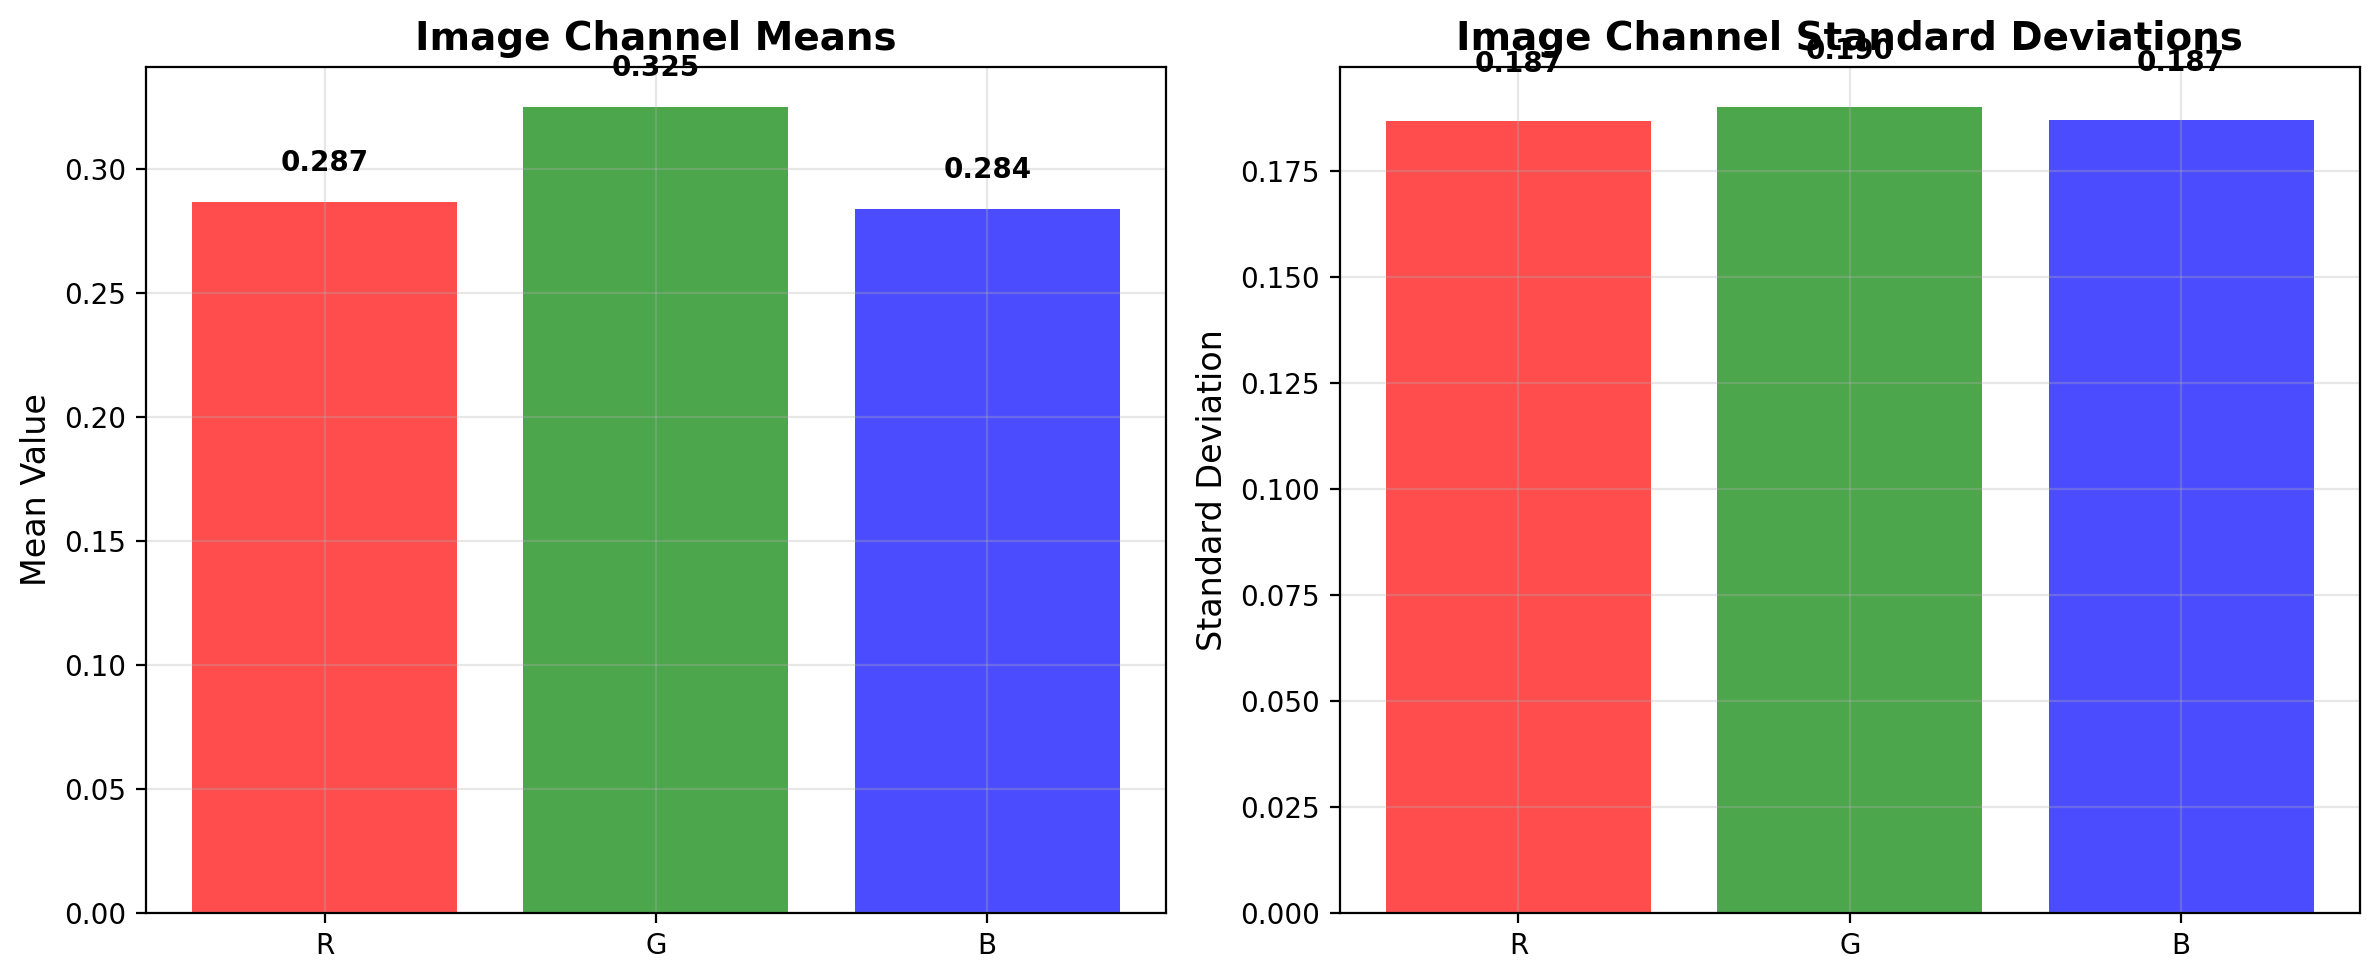
\includegraphics[width=\textwidth]{result/analysis/cityscapes_mean_std.png}  
    % 图片标题
    \caption{cityscapes数据集图像均值与标准差}
    \label{fig:mean_std}
\end{figure}
\begin{figure}[H]  % htbp表示此图片可浮动在合适位置
    \centering        % 图片居中
    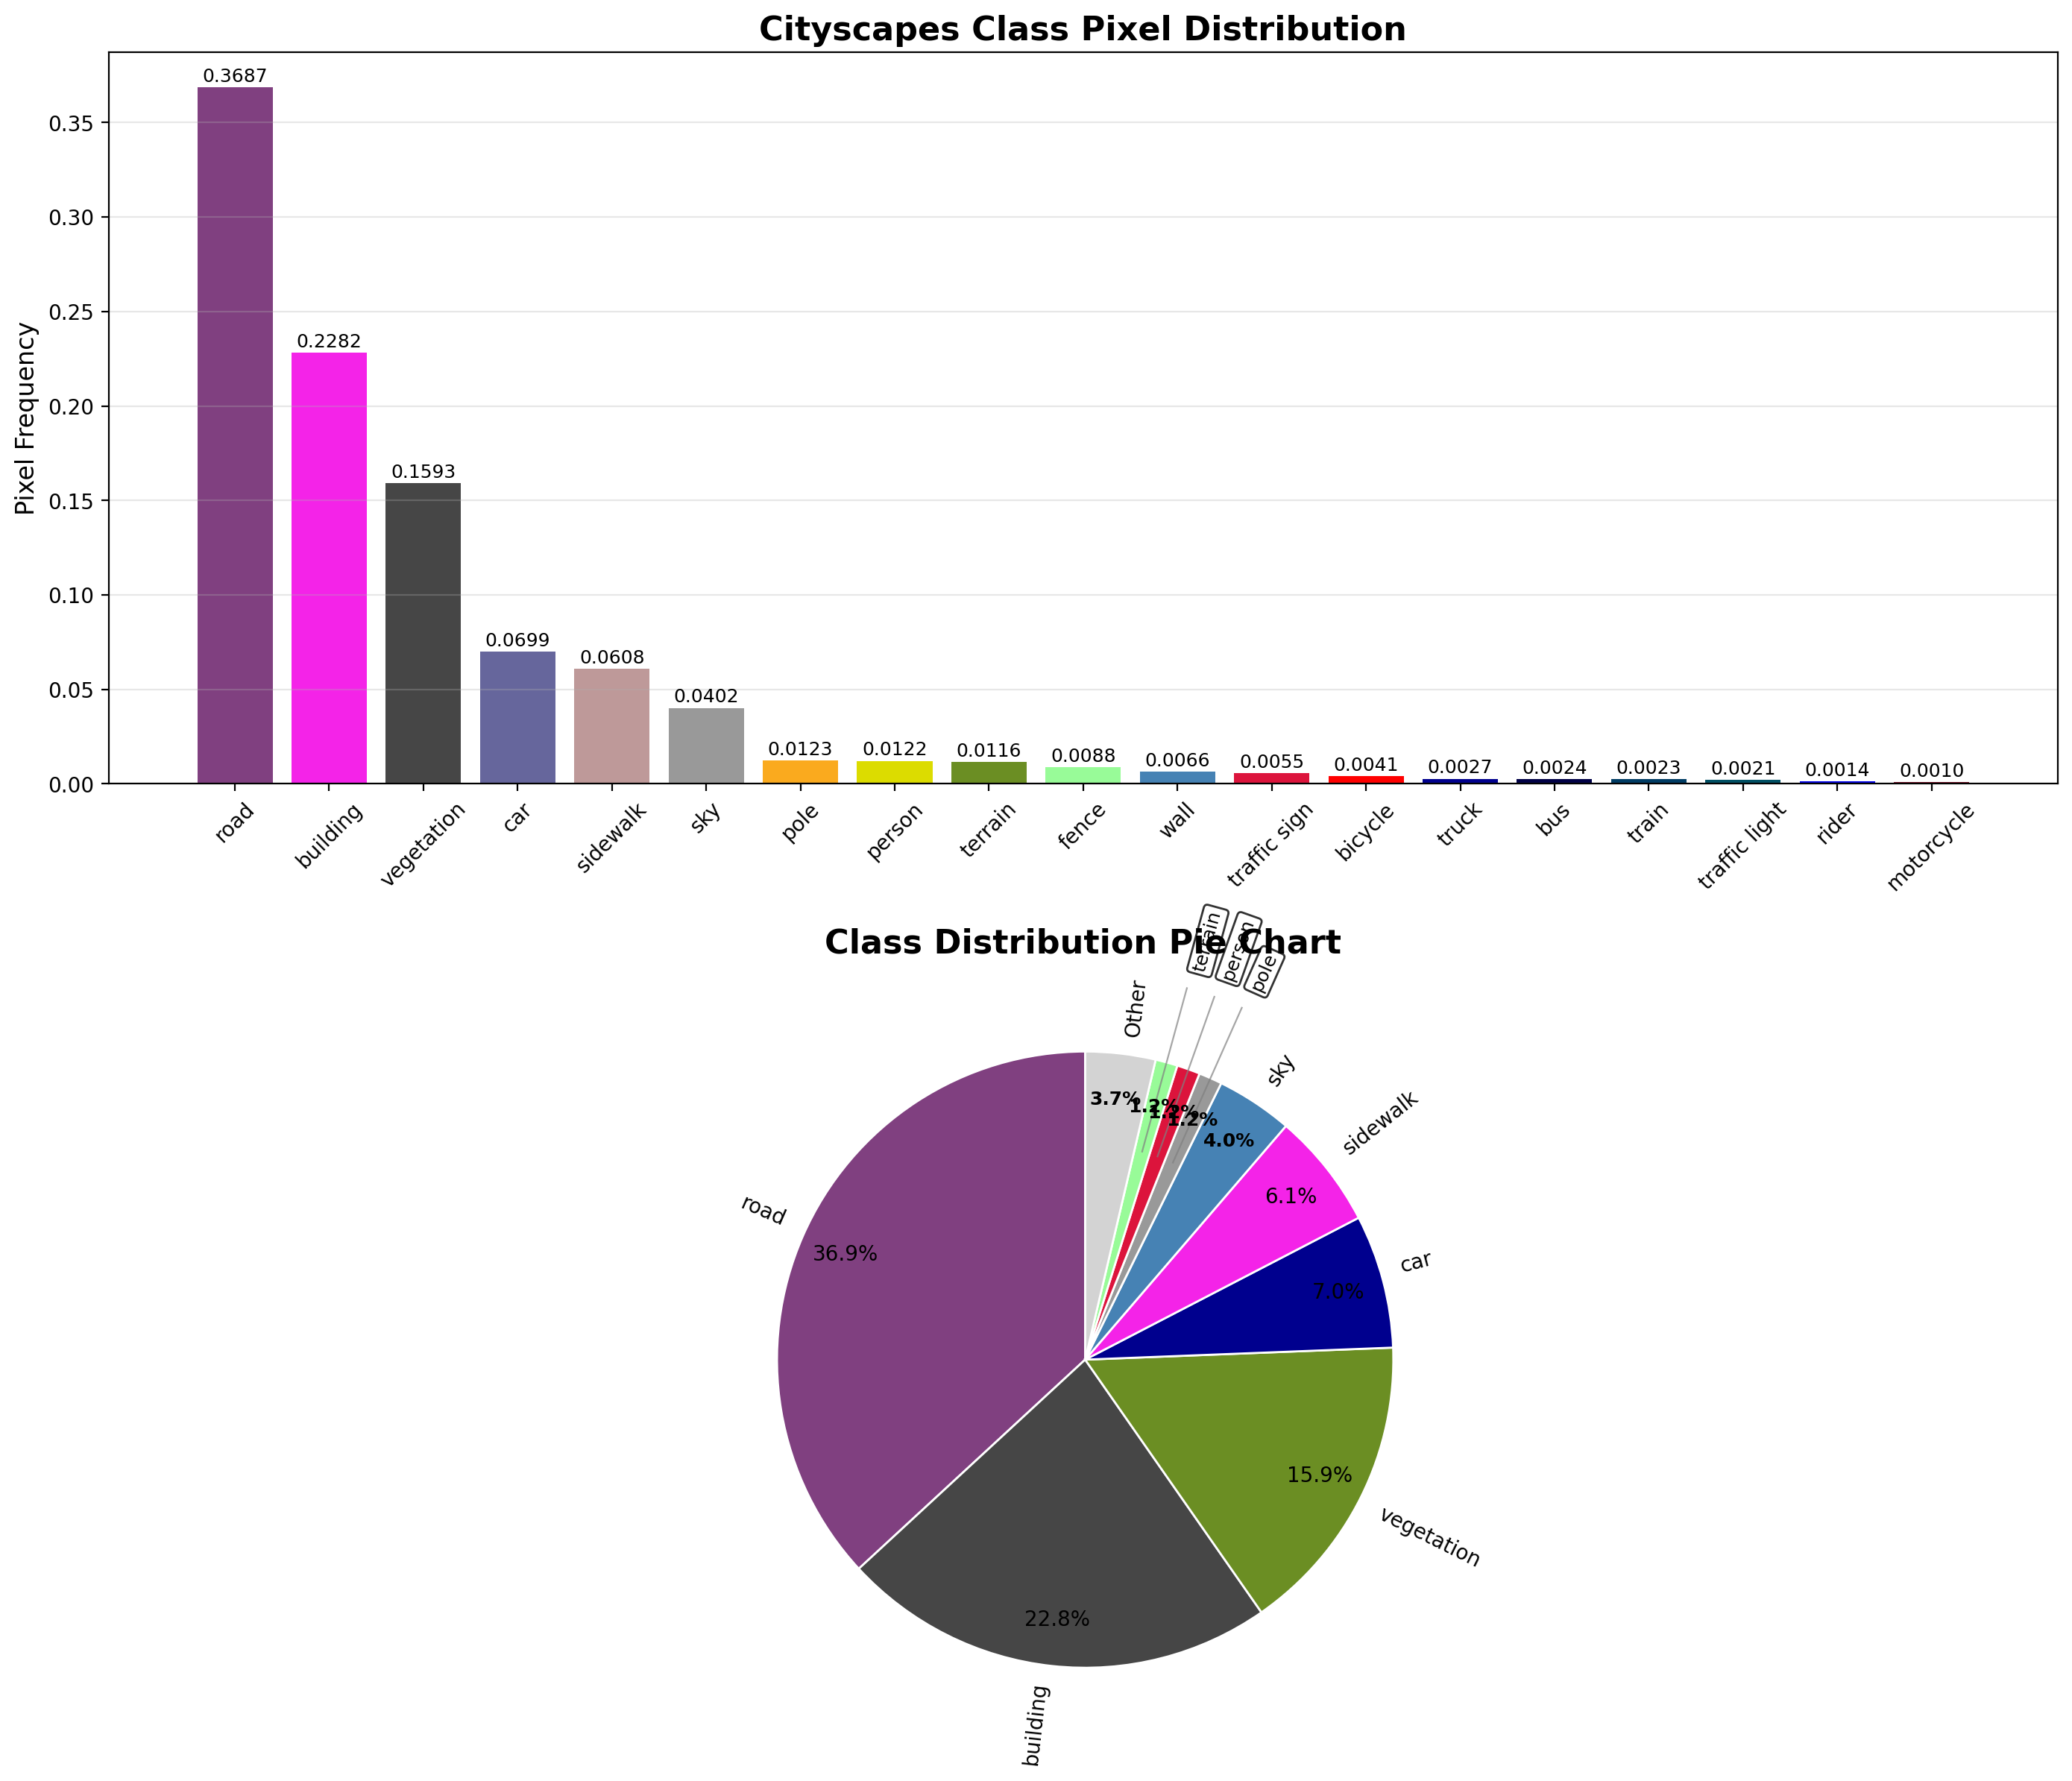
\includegraphics[width=\textwidth]{result/analysis/cityscapes_class_distribution.png}  
    % 图片标题
    \caption{cityscapes数据集各类别占比}
    \label{fig:class_distribution}
\end{figure}

\subsection{数据集处理}
下载好cityscapes数据集后解压,放到 ..../mmsegmentation/data/中,运行\newline
\verb|python tools/dataset_converters/cityscapes.py ./data/cityscapes --nproc 8| \newline
对数据集进行处理,之后就可以进行训练了。

对于图像裁切,翻转,尺度变换等数据增强甚至光照变化都在mmsegmentation的./config/\_base\_/datasets/cityscapes.py中进行了定义。
\begin{lstlisting}[language=Python]
# dataset settings
dataset_type = 'CityscapesDataset'
data_root = 'data/cityscapes/'
crop_size = (512, 1024)
train_pipeline = [
    dict(type='LoadImageFromFile'),
    dict(type='LoadAnnotations'),
    dict(
        type='RandomResize',
        scale=(2048, 1024),
        ratio_range=(0.5, 2.0),
        keep_ratio=True),
    dict(type='RandomCrop', crop_size=crop_size, cat_max_ratio=0.75),
    dict(type='RandomFlip', prob=0.5),
    dict(type='PhotoMetricDistortion'),
    dict(type='PackSegInputs')
]
\end{lstlisting}


\subsection{deeplabv3plus的训练,测试与可视化}
1. 开始训练

使用deeplabv3plus\_r50-d8\_4xb2-80k\_cityscapes-512x1024.py
进行训练。
训练结果如下:
\begin{lstlisting}[language=bash]
+---------------+-------+-------+
|     Class     |  IoU  |  Acc  |
+---------------+-------+-------+
|      road     | 96.46 |  97.5 |
|    sidewalk   | 80.23 | 89.45 |
|    building   | 88.73 | 95.47 |
|      wall     | 34.81 | 37.31 |
|     fence     | 51.58 | 65.53 |
|      pole     | 59.78 |  74.3 |
| traffic light | 64.04 | 77.32 |
|  traffic sign | 72.82 |  81.9 |
|   vegetation  |  91.0 |  96.6 |
|    terrain    | 56.71 | 63.49 |
|      sky      | 93.27 | 97.52 |
|     person    |  77.4 | 86.94 |
|     rider     | 53.55 | 78.05 |
|      car      | 92.94 | 97.23 |
|     truck     | 50.72 | 68.15 |
|      bus      | 56.41 | 62.71 |
|     train     | 35.35 |  41.1 |
|   motorcycle  | 45.51 |  52.7 |
|    bicycle    | 70.84 | 83.11 |
+---------------+-------+-------+
10/24 01:14:40 - mmengine - INFO - Iter(val) [500/500]    aAcc: 94.3700  mIoU: 66.9600  mAcc: 76.1200  data_time: 0.0099  time: 0.1673
\end{lstlisting}

\begin{figure}[htbp]  % htbp表示此图片可浮动在合适位置
    \centering        % 图片居中
    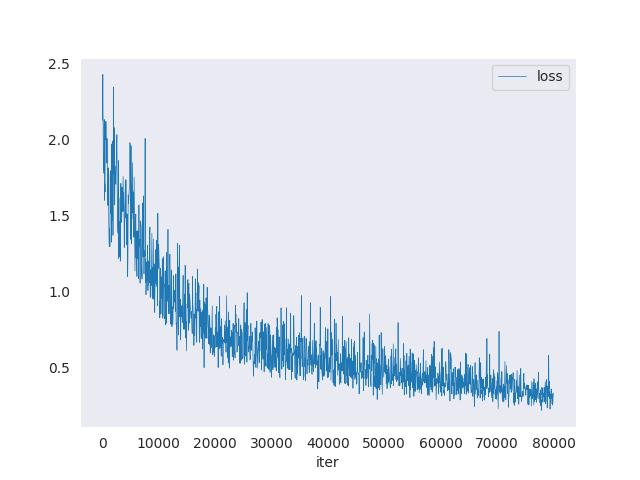
\includegraphics[width=0.49\textwidth]{result/plot/loss_deeplabv3plus.jpg}
    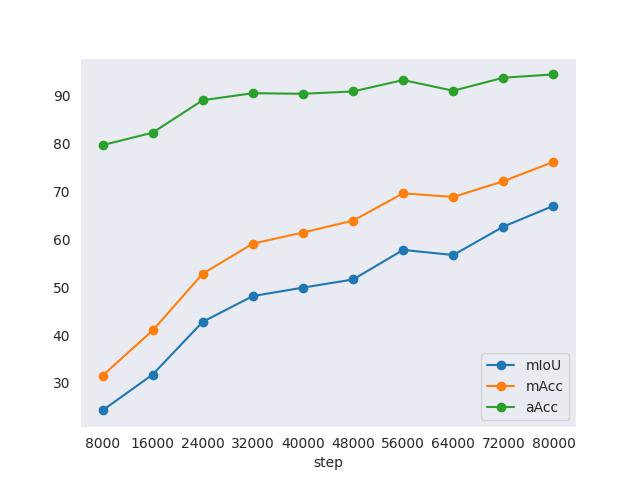
\includegraphics[width=0.49\textwidth]{result/plot/acc_deeplabv3plus.jpg} 
    % 图片标题
    \caption{deeplabv3plus模型的loss曲线(左)与mIoU曲线(右)}
    \label{fig:loss_acc_deeplabv3plus}
\end{figure}
分割结果展示如下:
\begin{figure}[htbp]  % htbp表示此图片可浮动在合适位置
    \centering        % 图片居中
    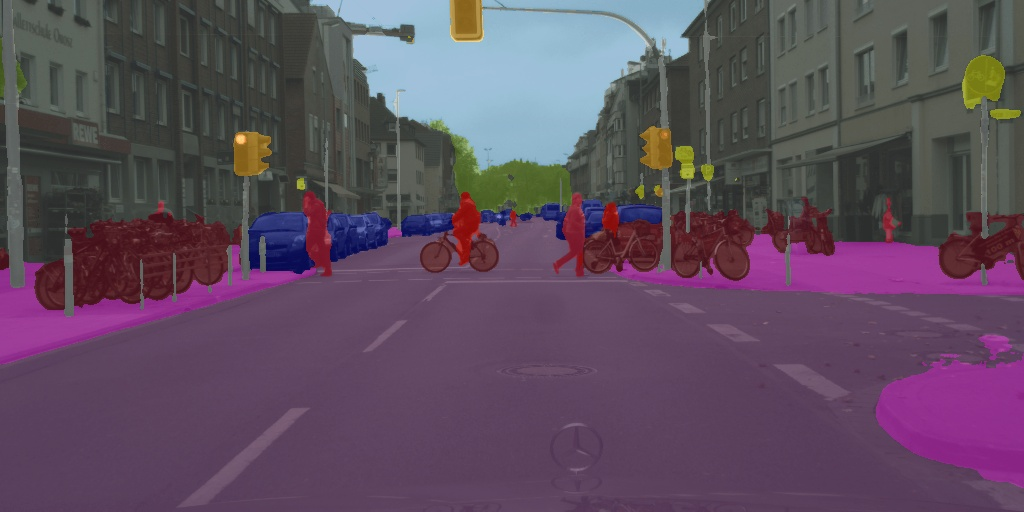
\includegraphics[width=0.49\textwidth]{result/plot/result_deeplabv3plus.jpg}
    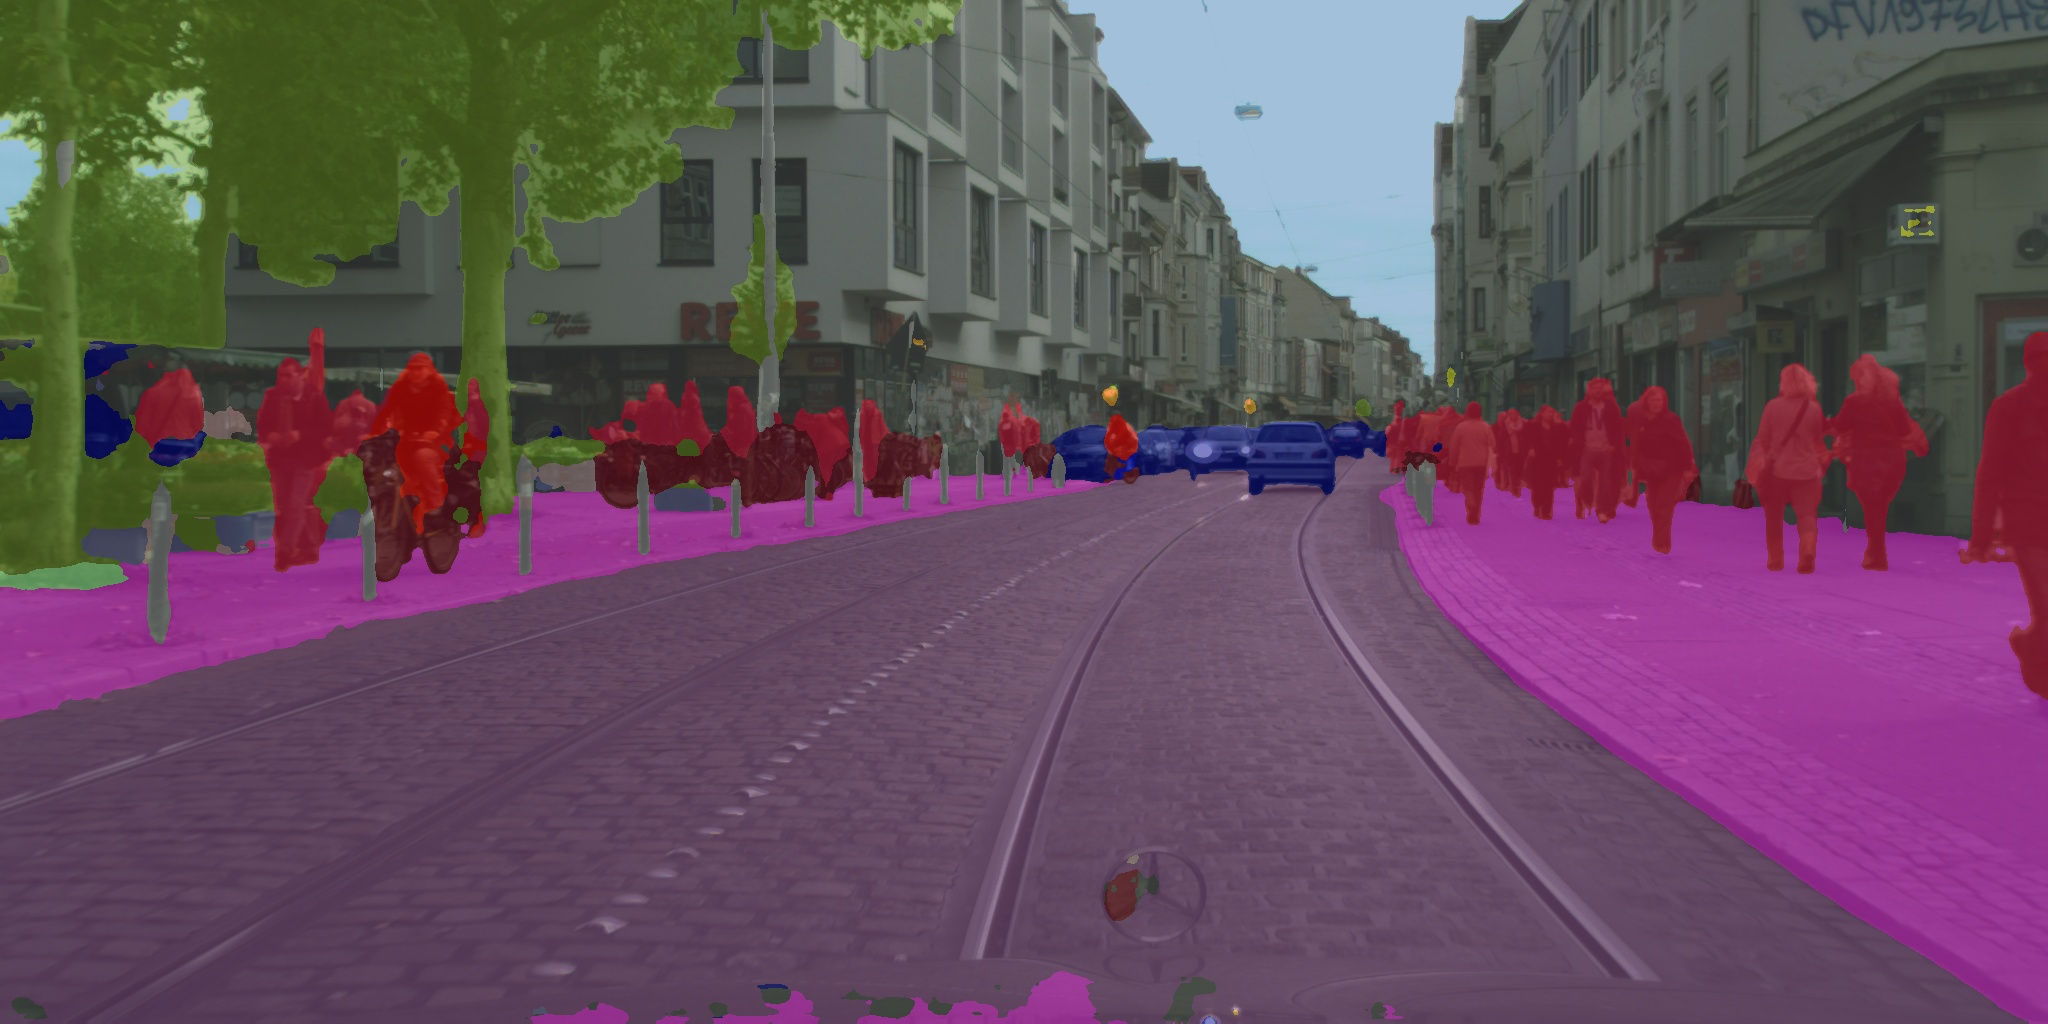
\includegraphics[width=0.49\textwidth]{result/plot/result_1_deeplabv3plus.jpg}
    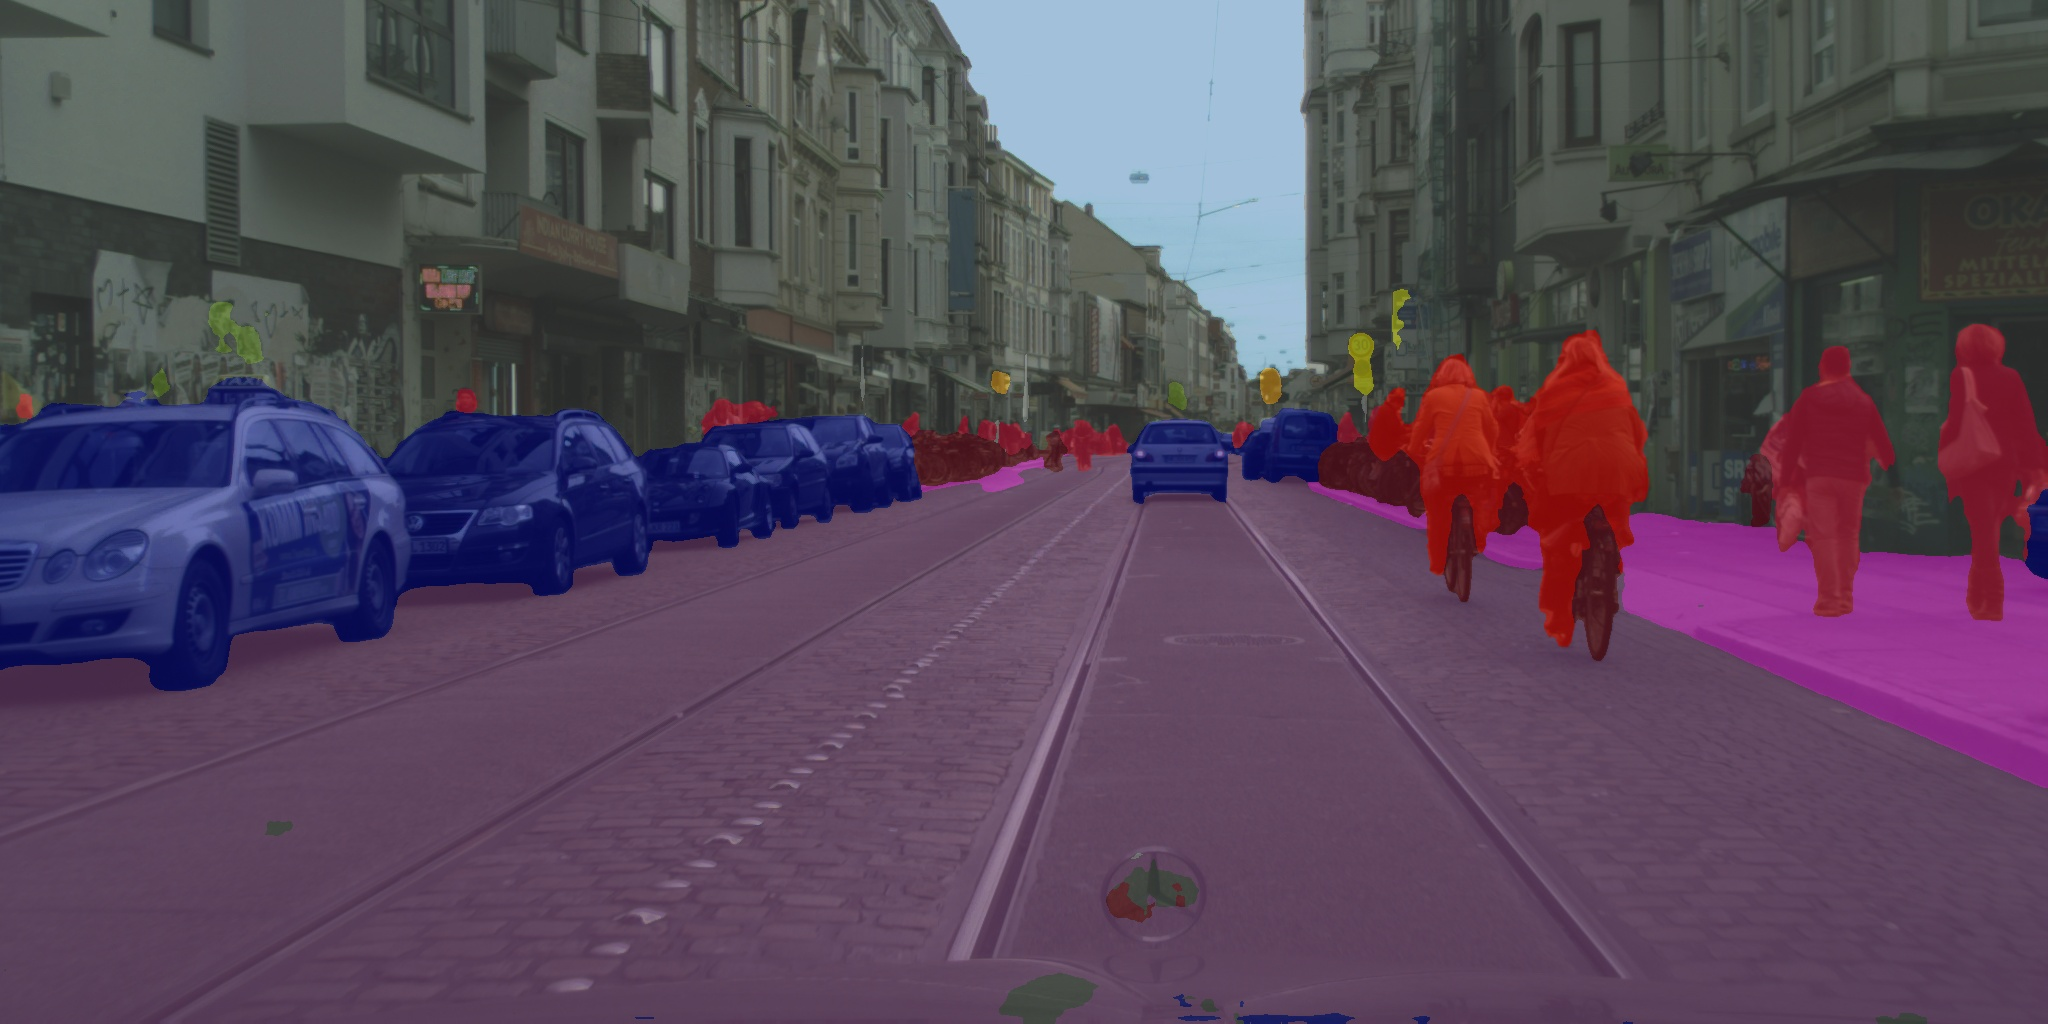
\includegraphics[width=0.49\textwidth]{result/plot/result_2_deeplabv3plus.jpg}
    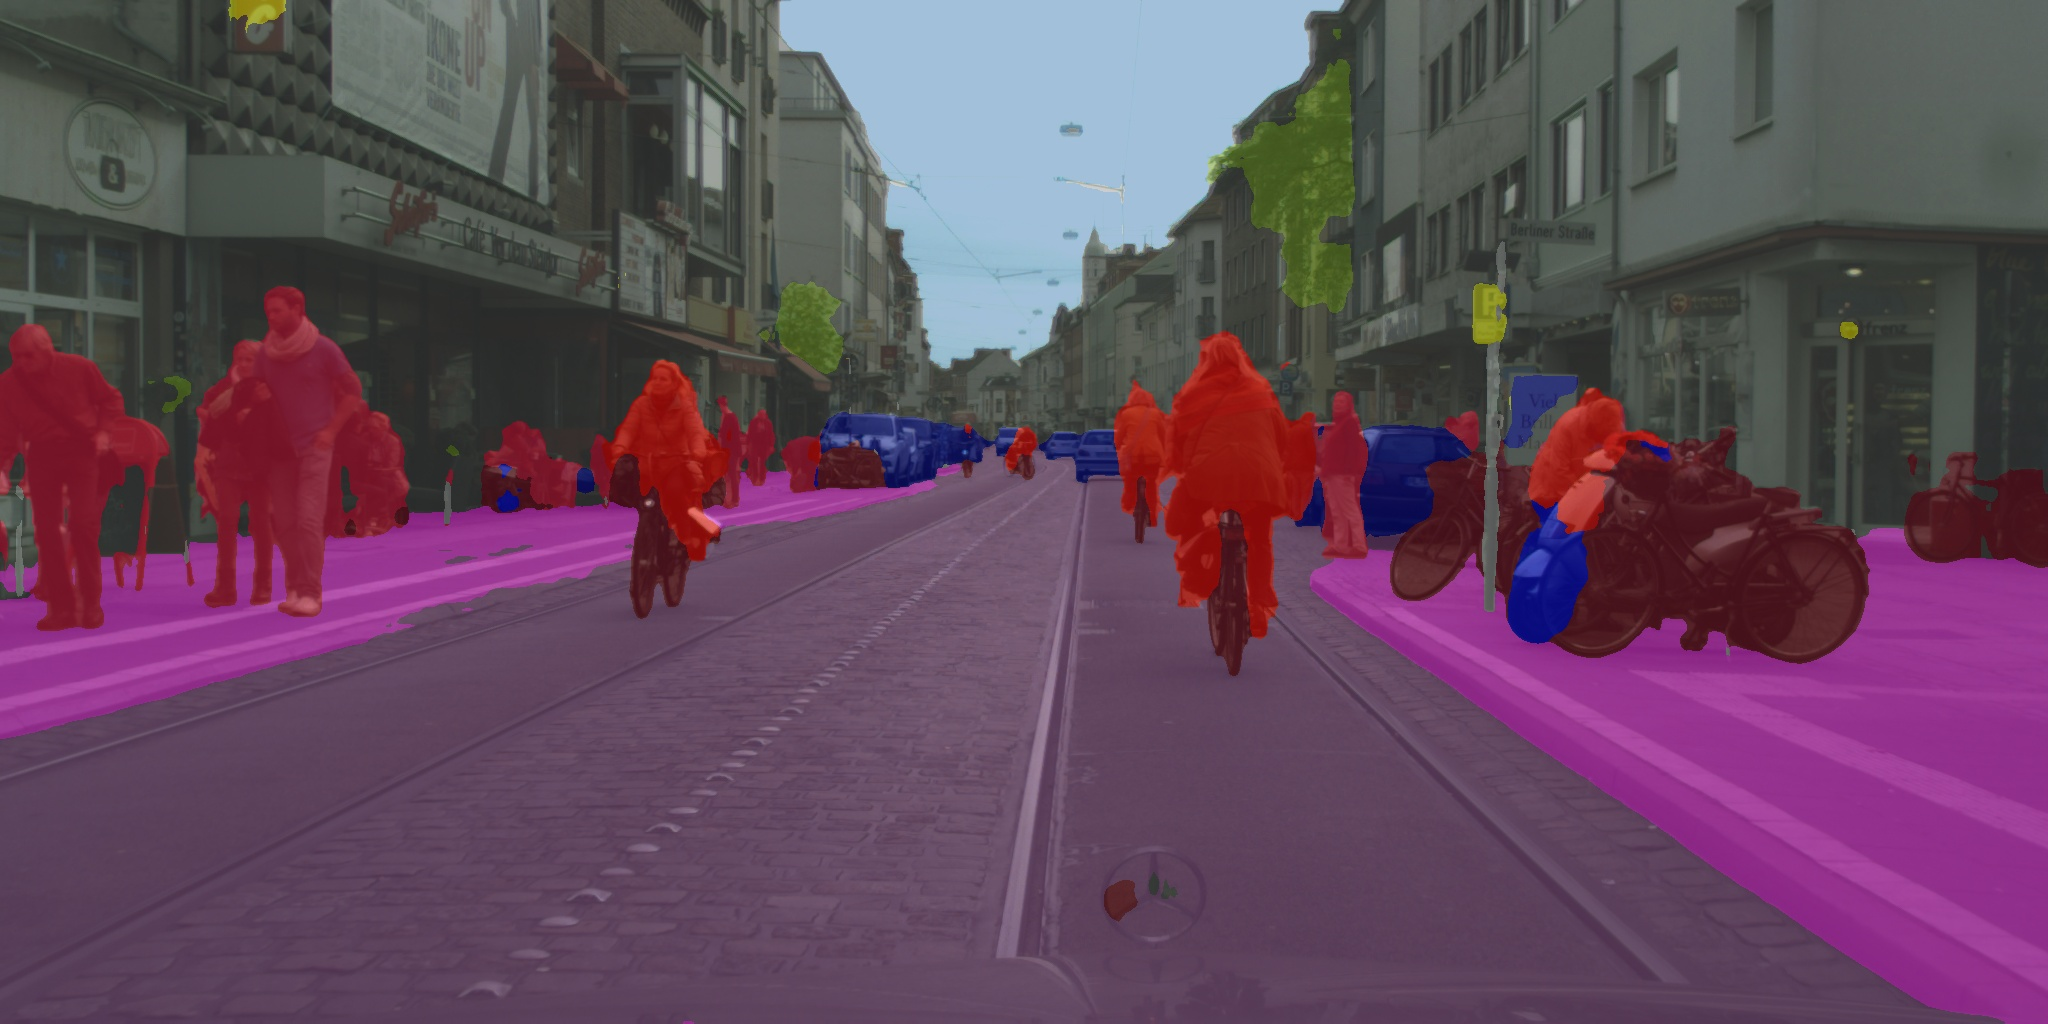
\includegraphics[width=0.49\textwidth]{result/plot/result_3_deeplabv3plus.jpg}
    % 图片标题
    \caption{deeplabv3plus模型的分割结果展示}
    \label{fig:result_deeplabv3plus}
\end{figure}
\begin{figure}[htbp]  % htbp表示此图片可浮动在合适位置
    \centering        % 图片居中
    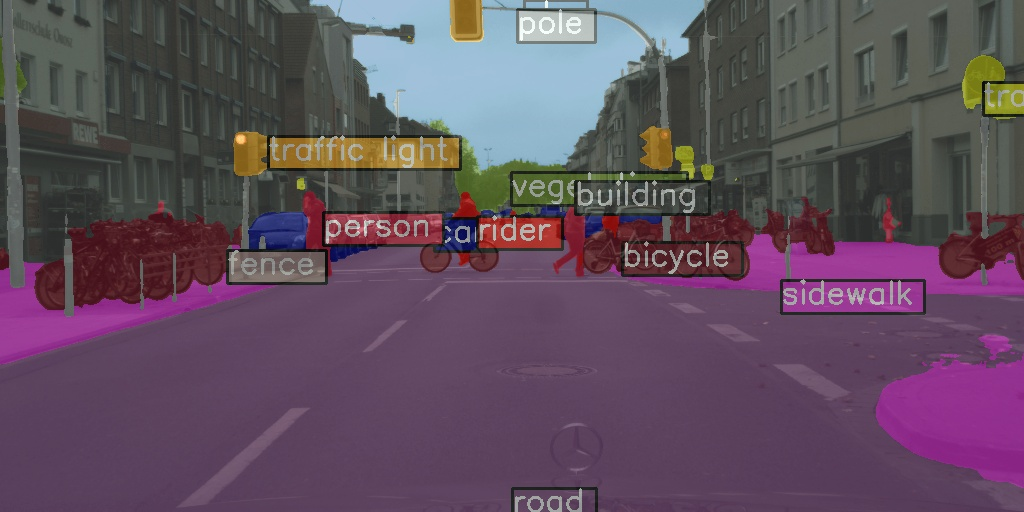
\includegraphics[width=0.49\textwidth]{result/plot/predict_deeplabv3plus.jpg}
    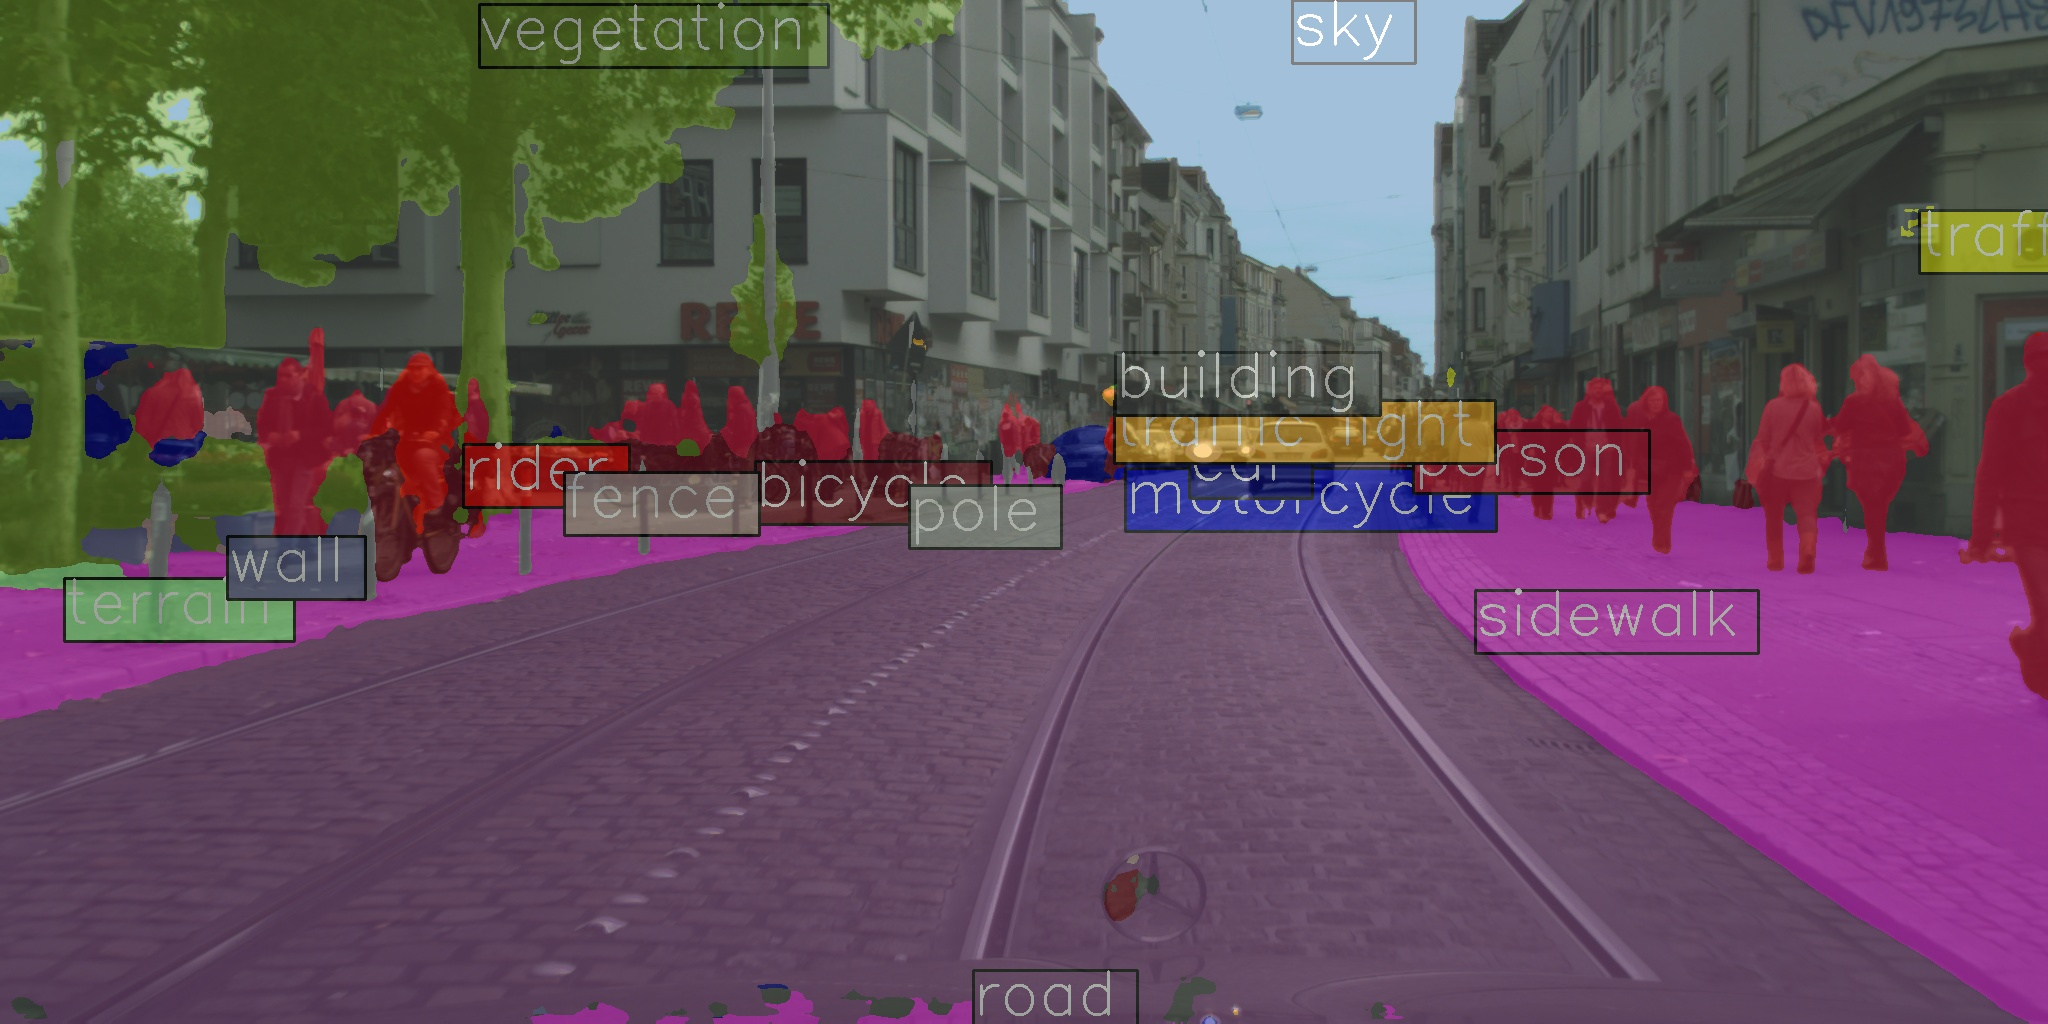
\includegraphics[width=0.49\textwidth]{result/plot/predict_1_deeplabv3plus.jpg}
    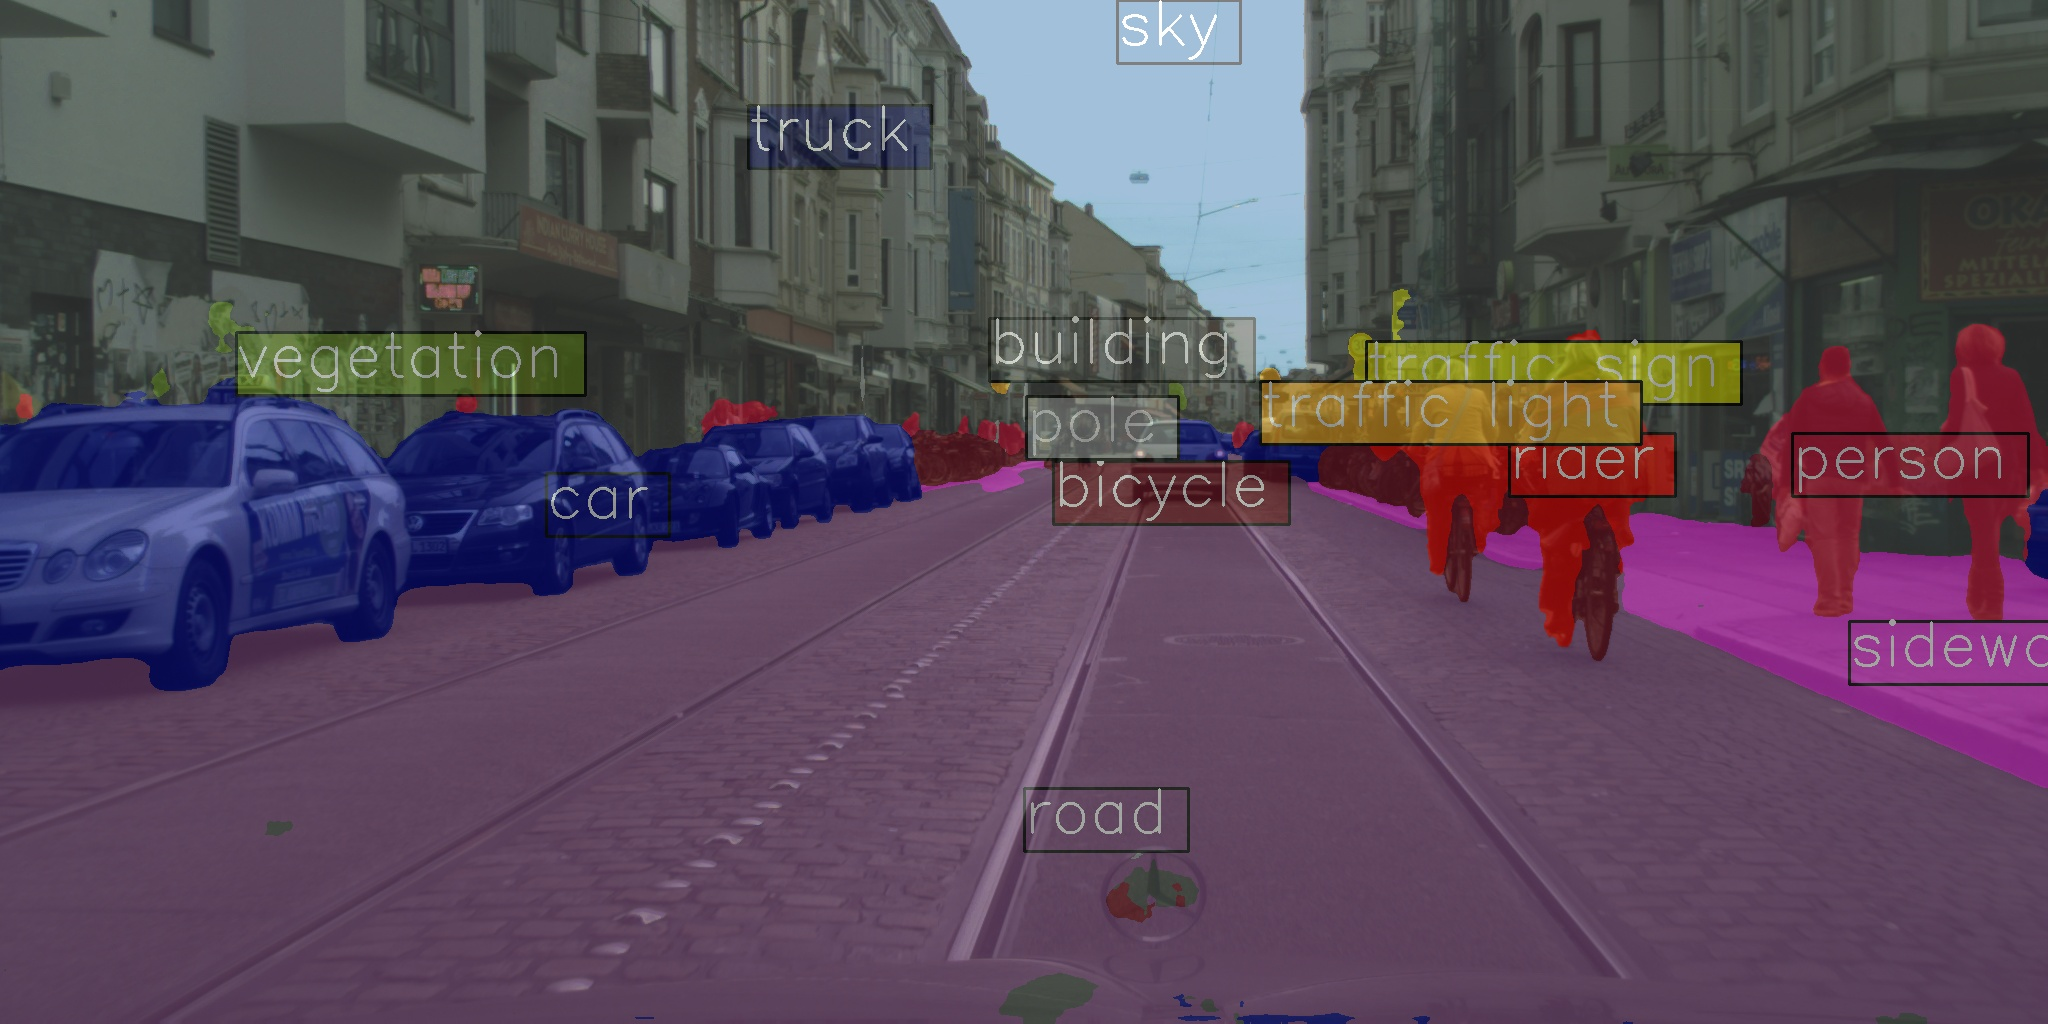
\includegraphics[width=0.49\textwidth]{result/plot/predict_2_deeplabv3plus.jpg}
    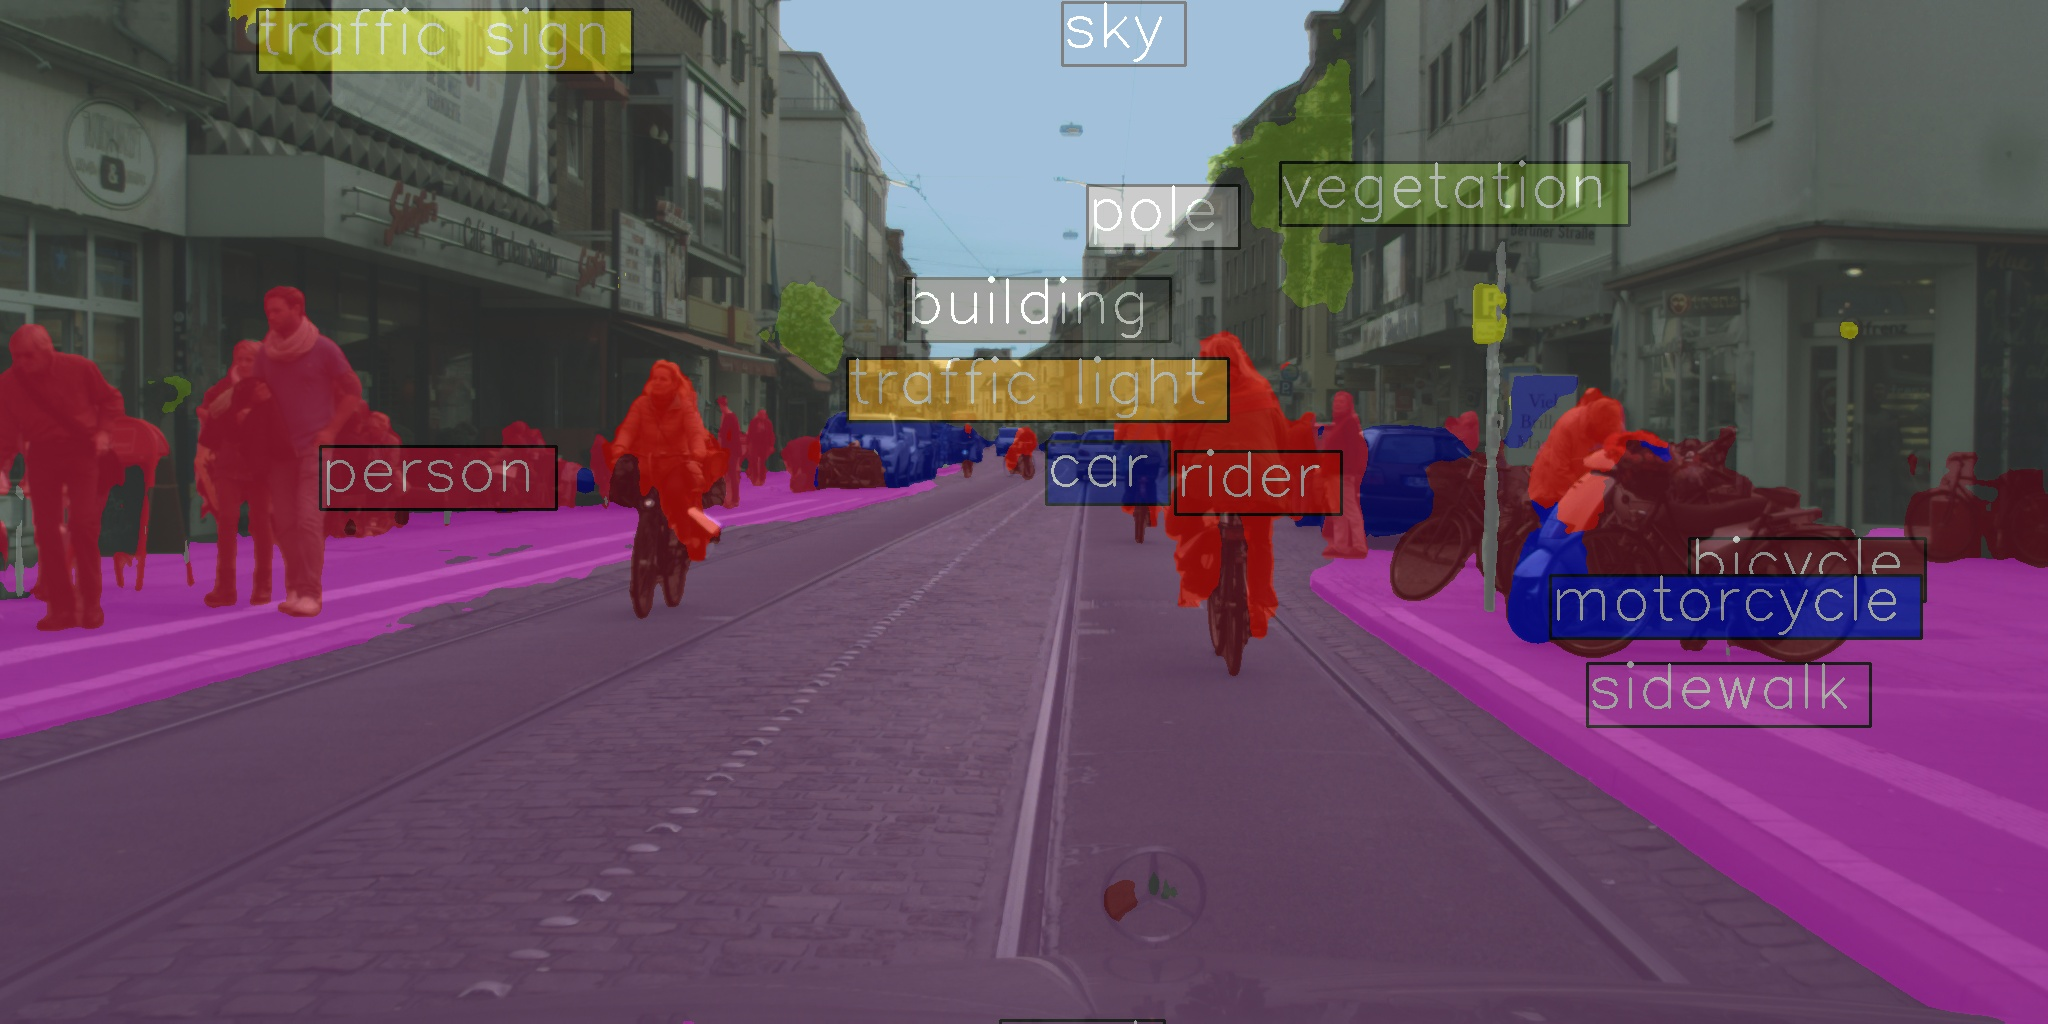
\includegraphics[width=0.49\textwidth]{result/plot/predict_3_deeplabv3plus.jpg}
    % 图片标题
    \caption{deeplabv3plus模型的预测结果展示}
    \label{fig:predict_deeplabv3plus}
\end{figure}
\begin{figure}[htbp]  % htbp表示此图片可浮动在合适位置
    \centering        % 图片居中
    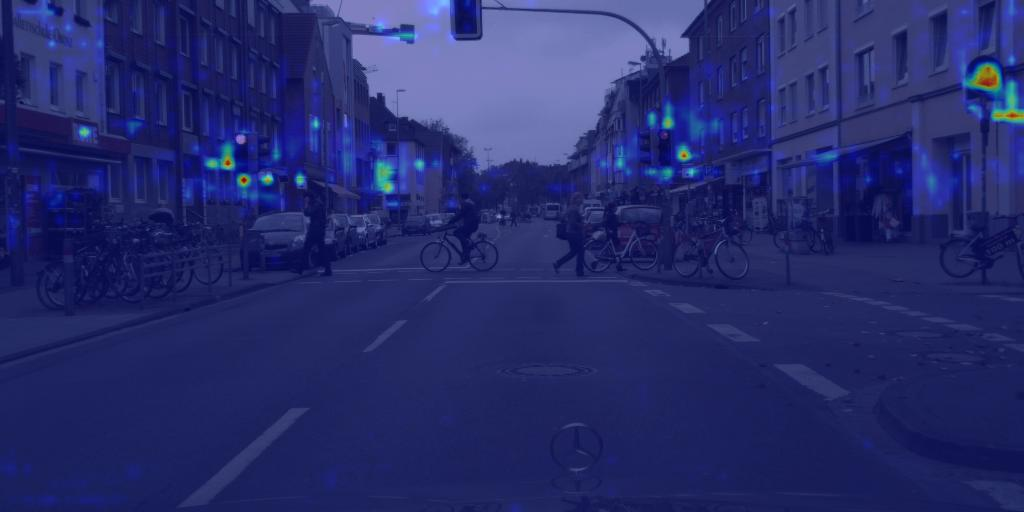
\includegraphics[width=0.49\textwidth]{result/plot/cam_deeplabv3plus.jpg}
    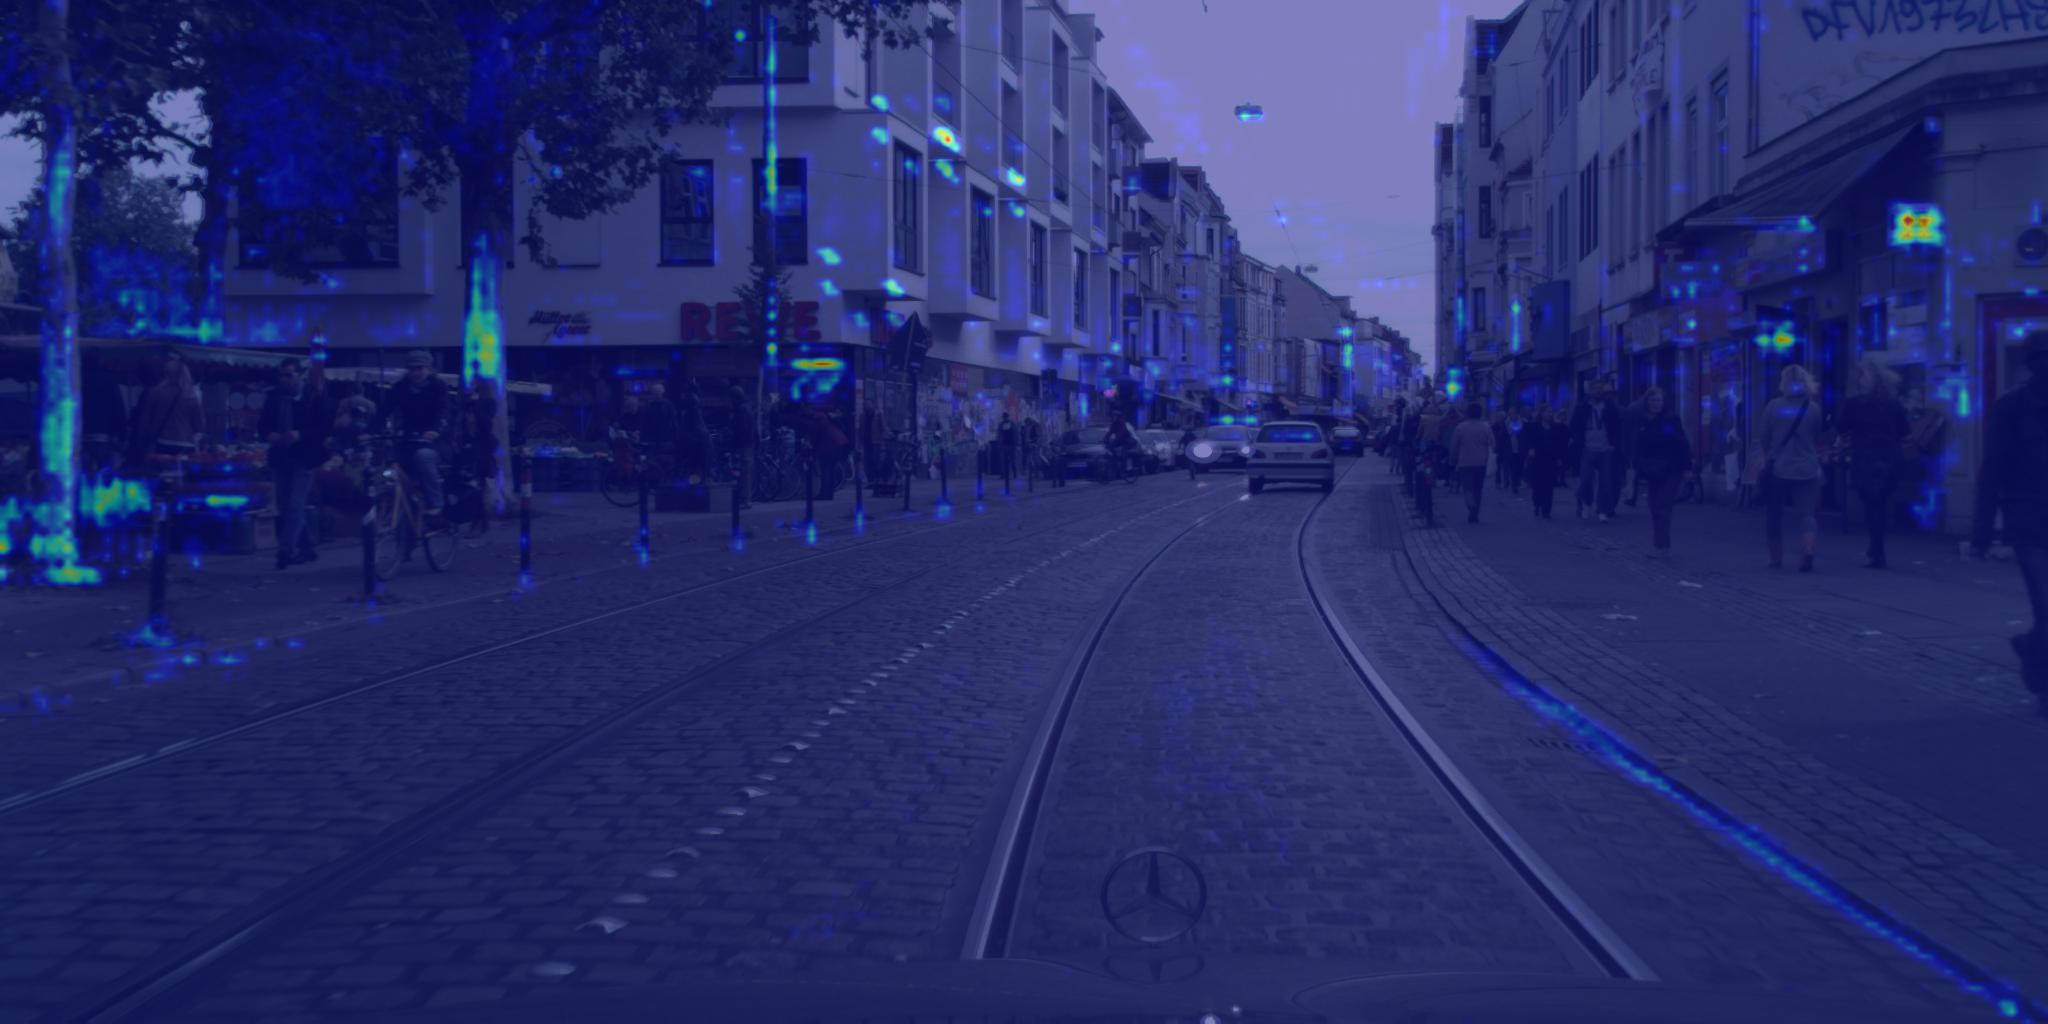
\includegraphics[width=0.49\textwidth]{result/plot/cam_1_deeplabv3plus.jpg}
    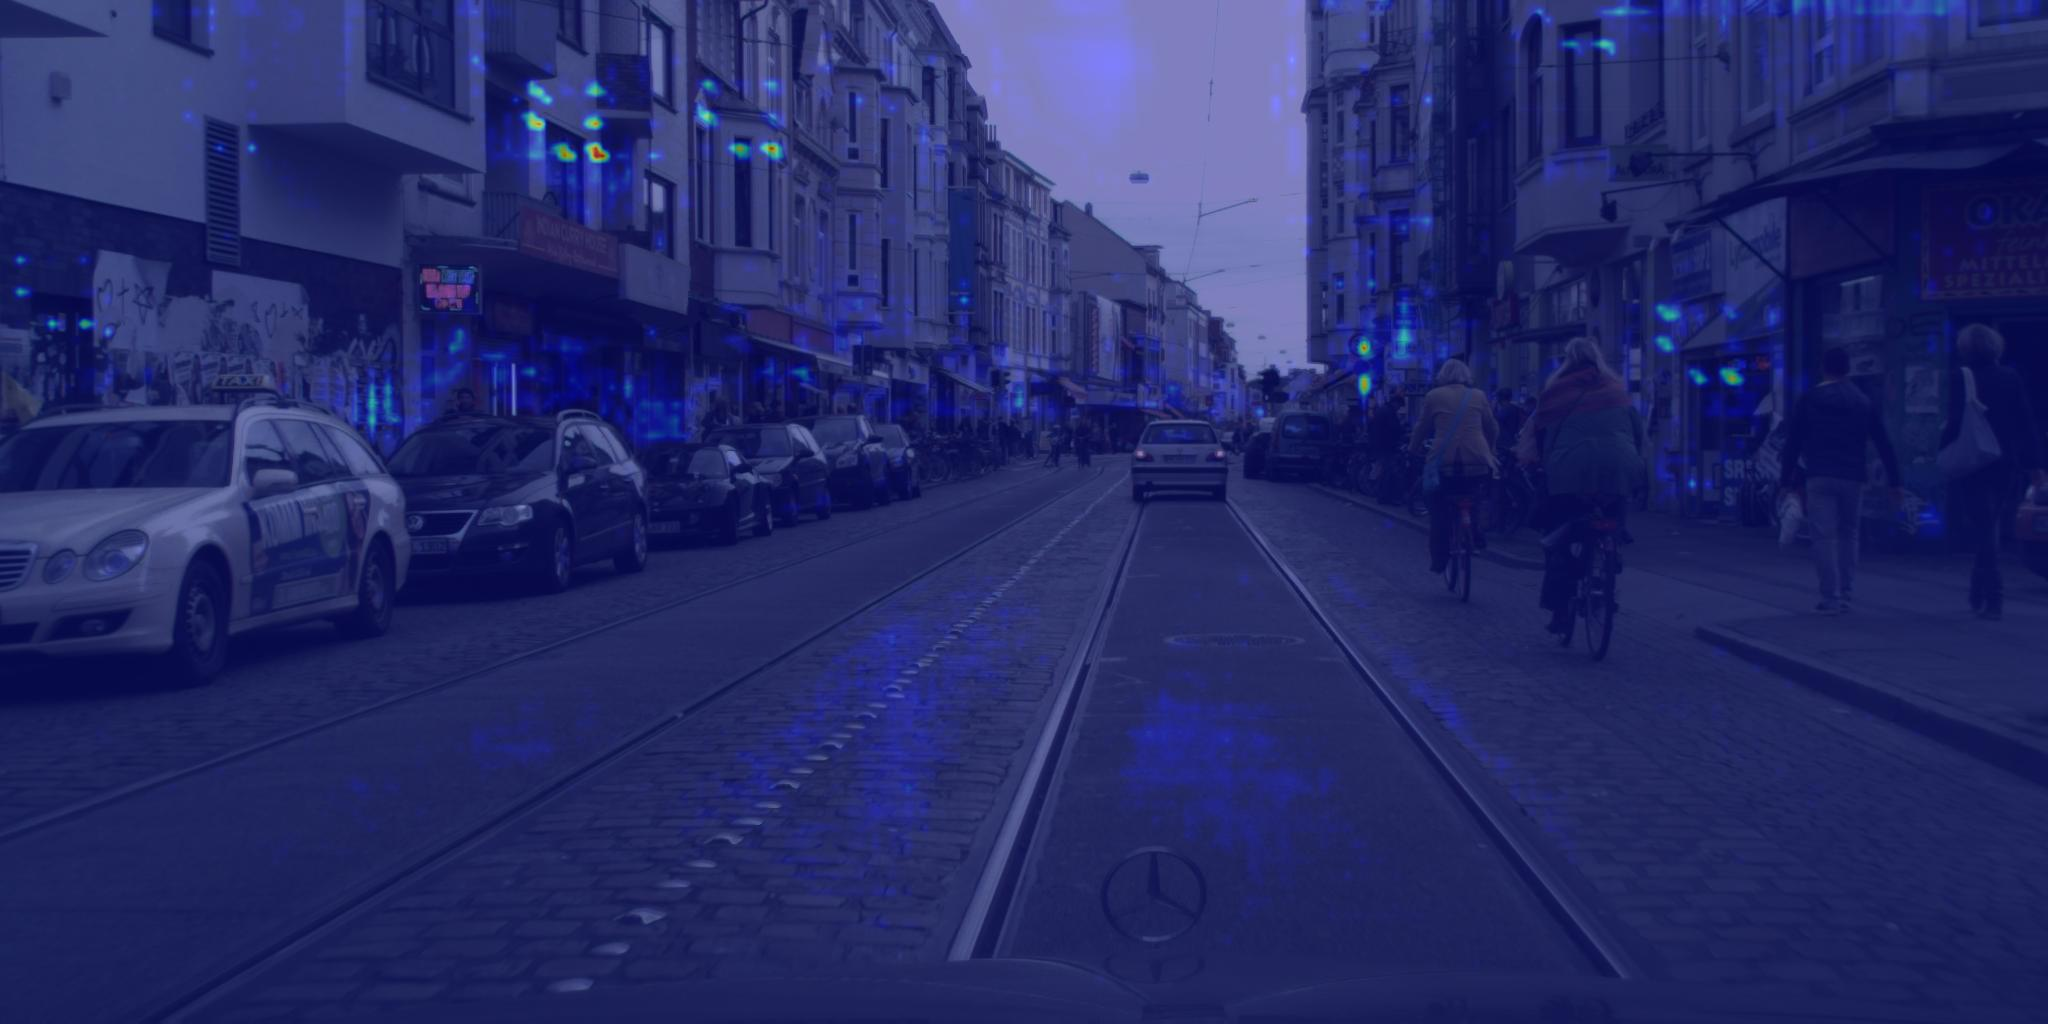
\includegraphics[width=0.49\textwidth]{result/plot/cam_2_deeplabv3plus.jpg}
    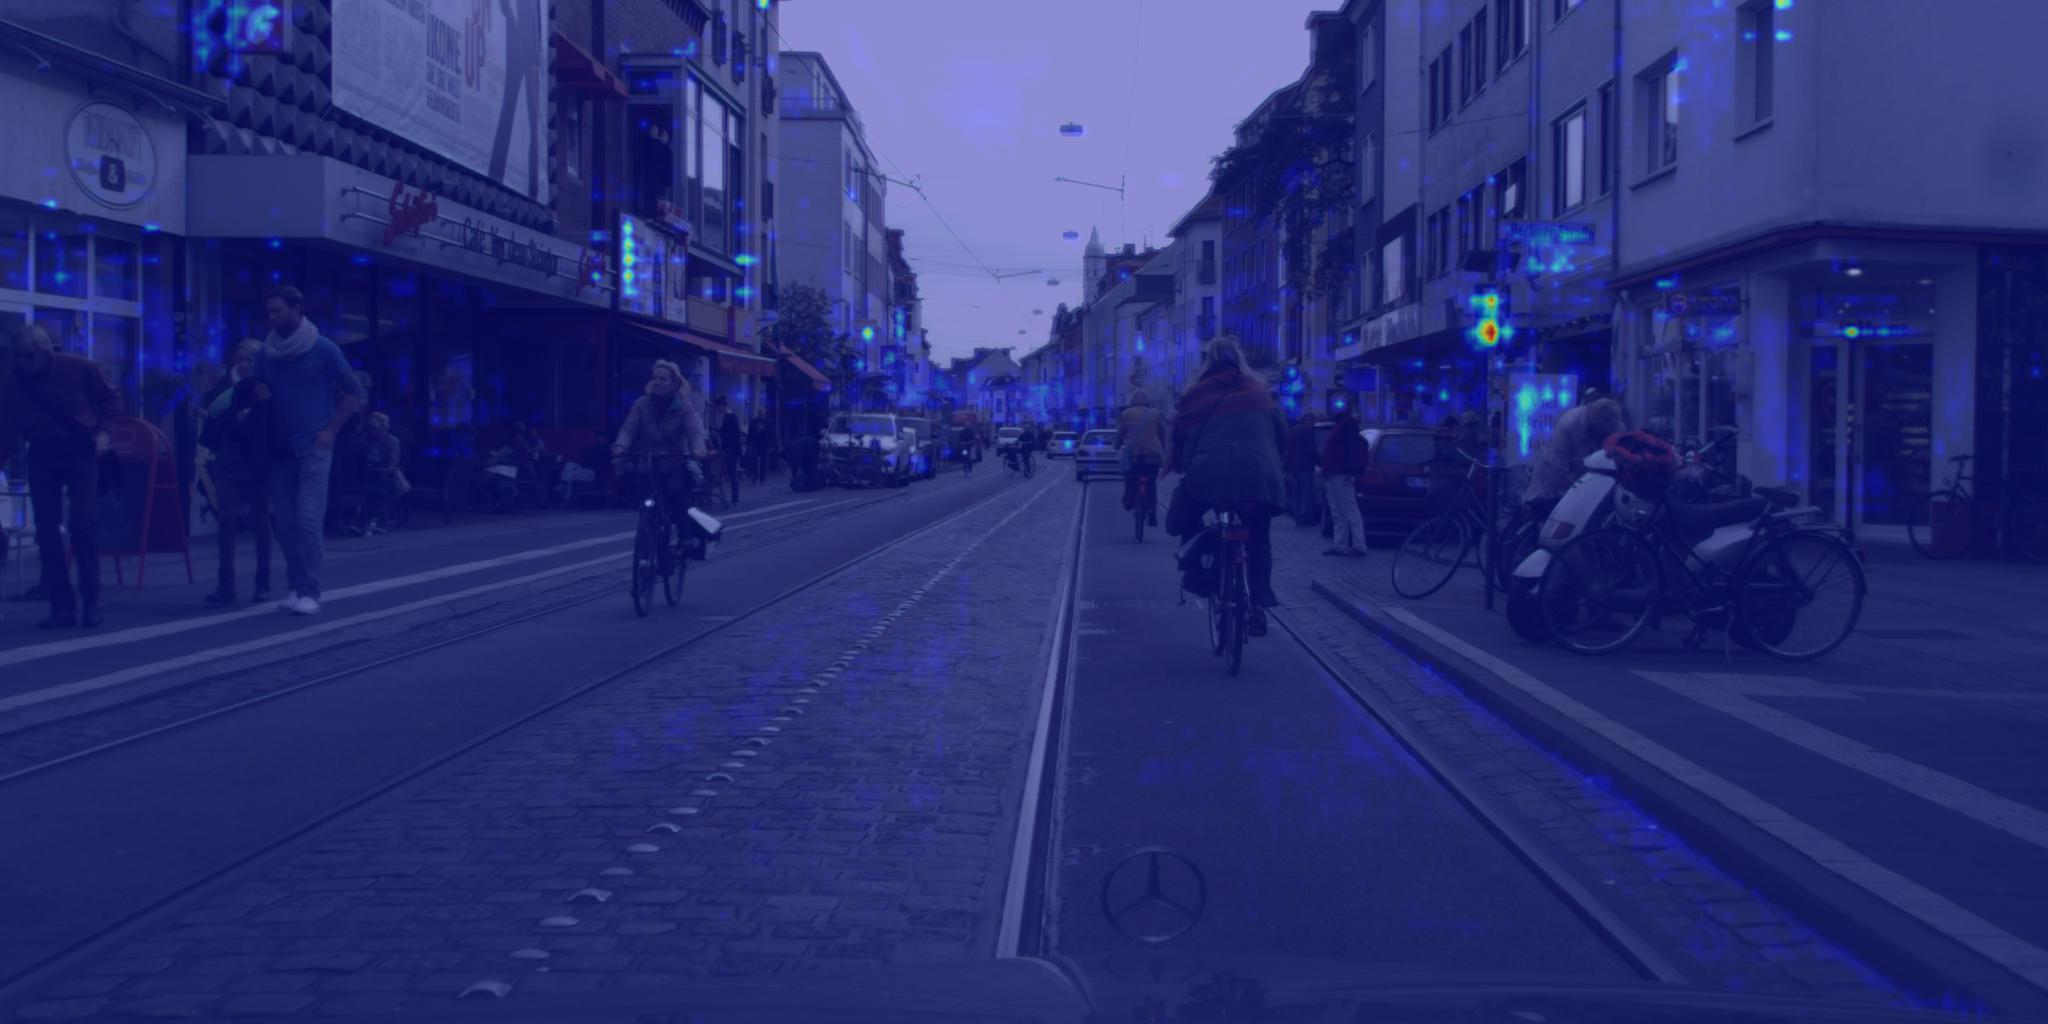
\includegraphics[width=0.49\textwidth]{result/plot/cam_3_deeplabv3plus.jpg}
    % 图片标题
    \caption{deeplabv3plus模型的cam图展示}
    \label{fig:cam_deeplabv3plus}
\end{figure}
\begin{figure}[H]  % htbp表示此图片可浮动在合适位置
    \centering        % 图片居中
    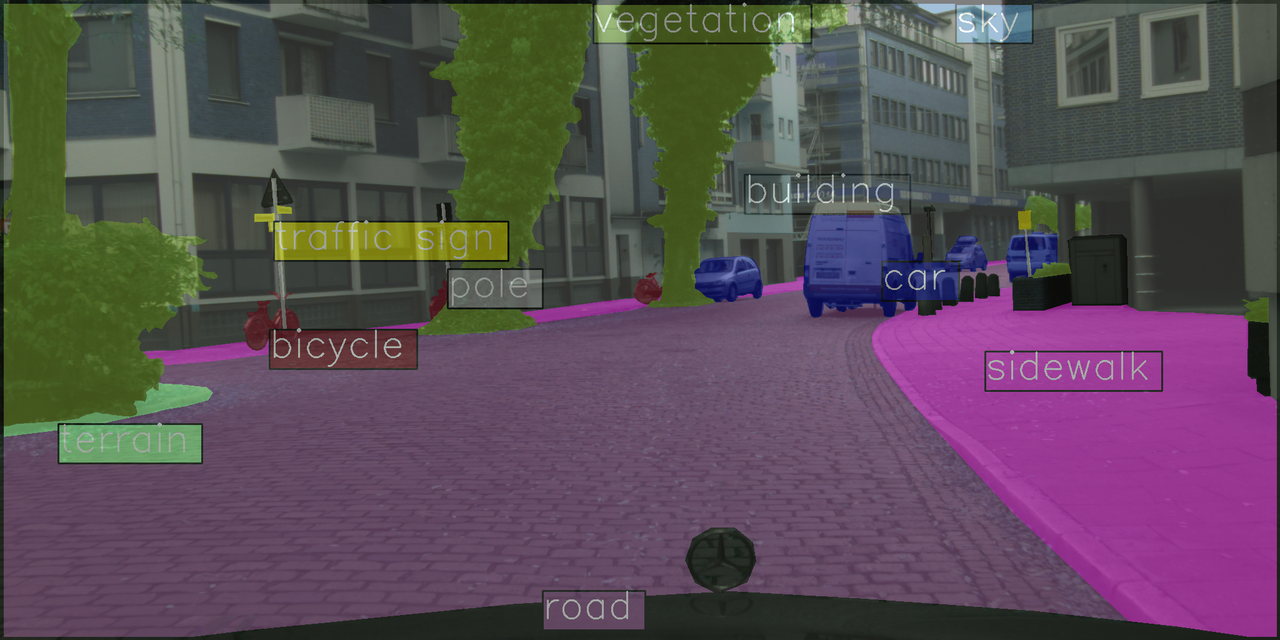
\includegraphics[width=0.49\textwidth]{result/plot/mask1.png}
    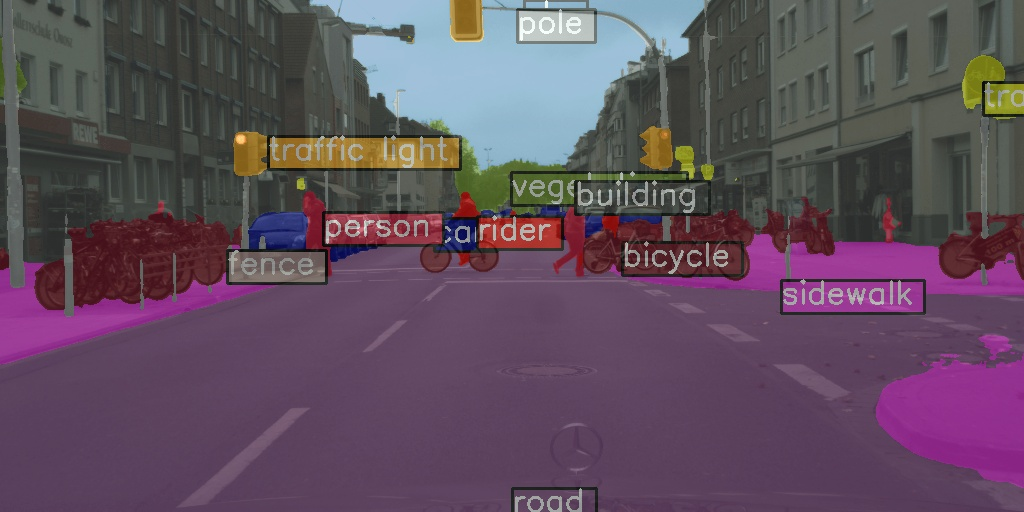
\includegraphics[width=0.49\textwidth]{result/plot/predict_deeplabv3plus.jpg}
    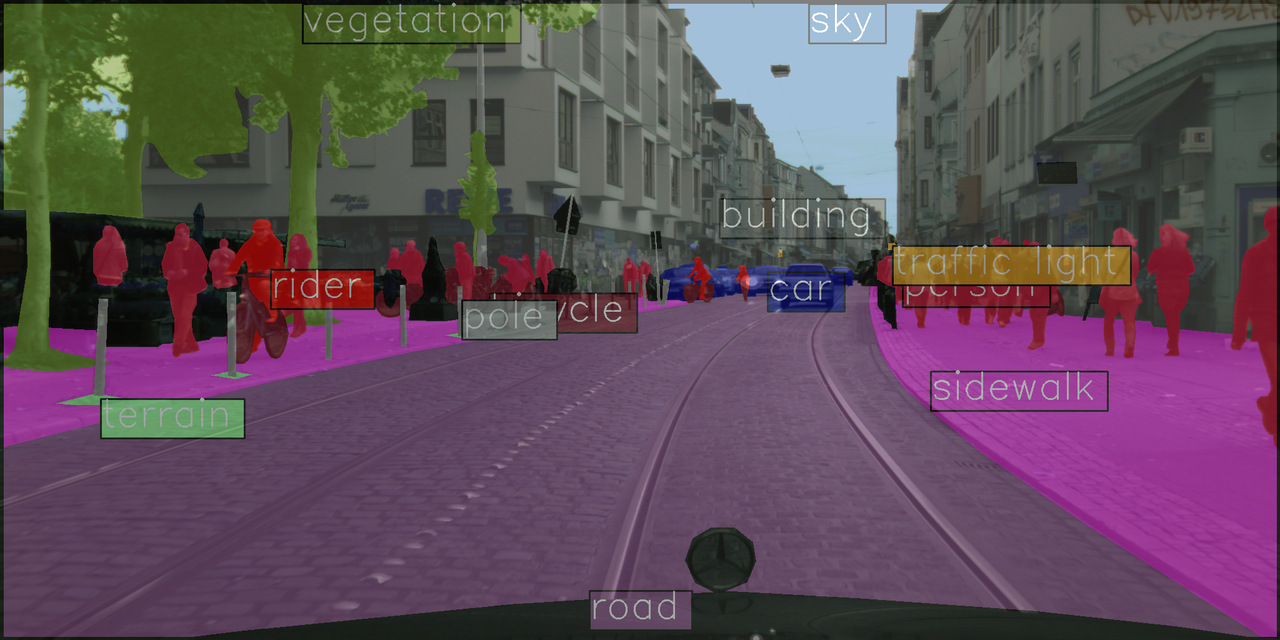
\includegraphics[width=0.49\textwidth]{result/plot/mask2.png}
    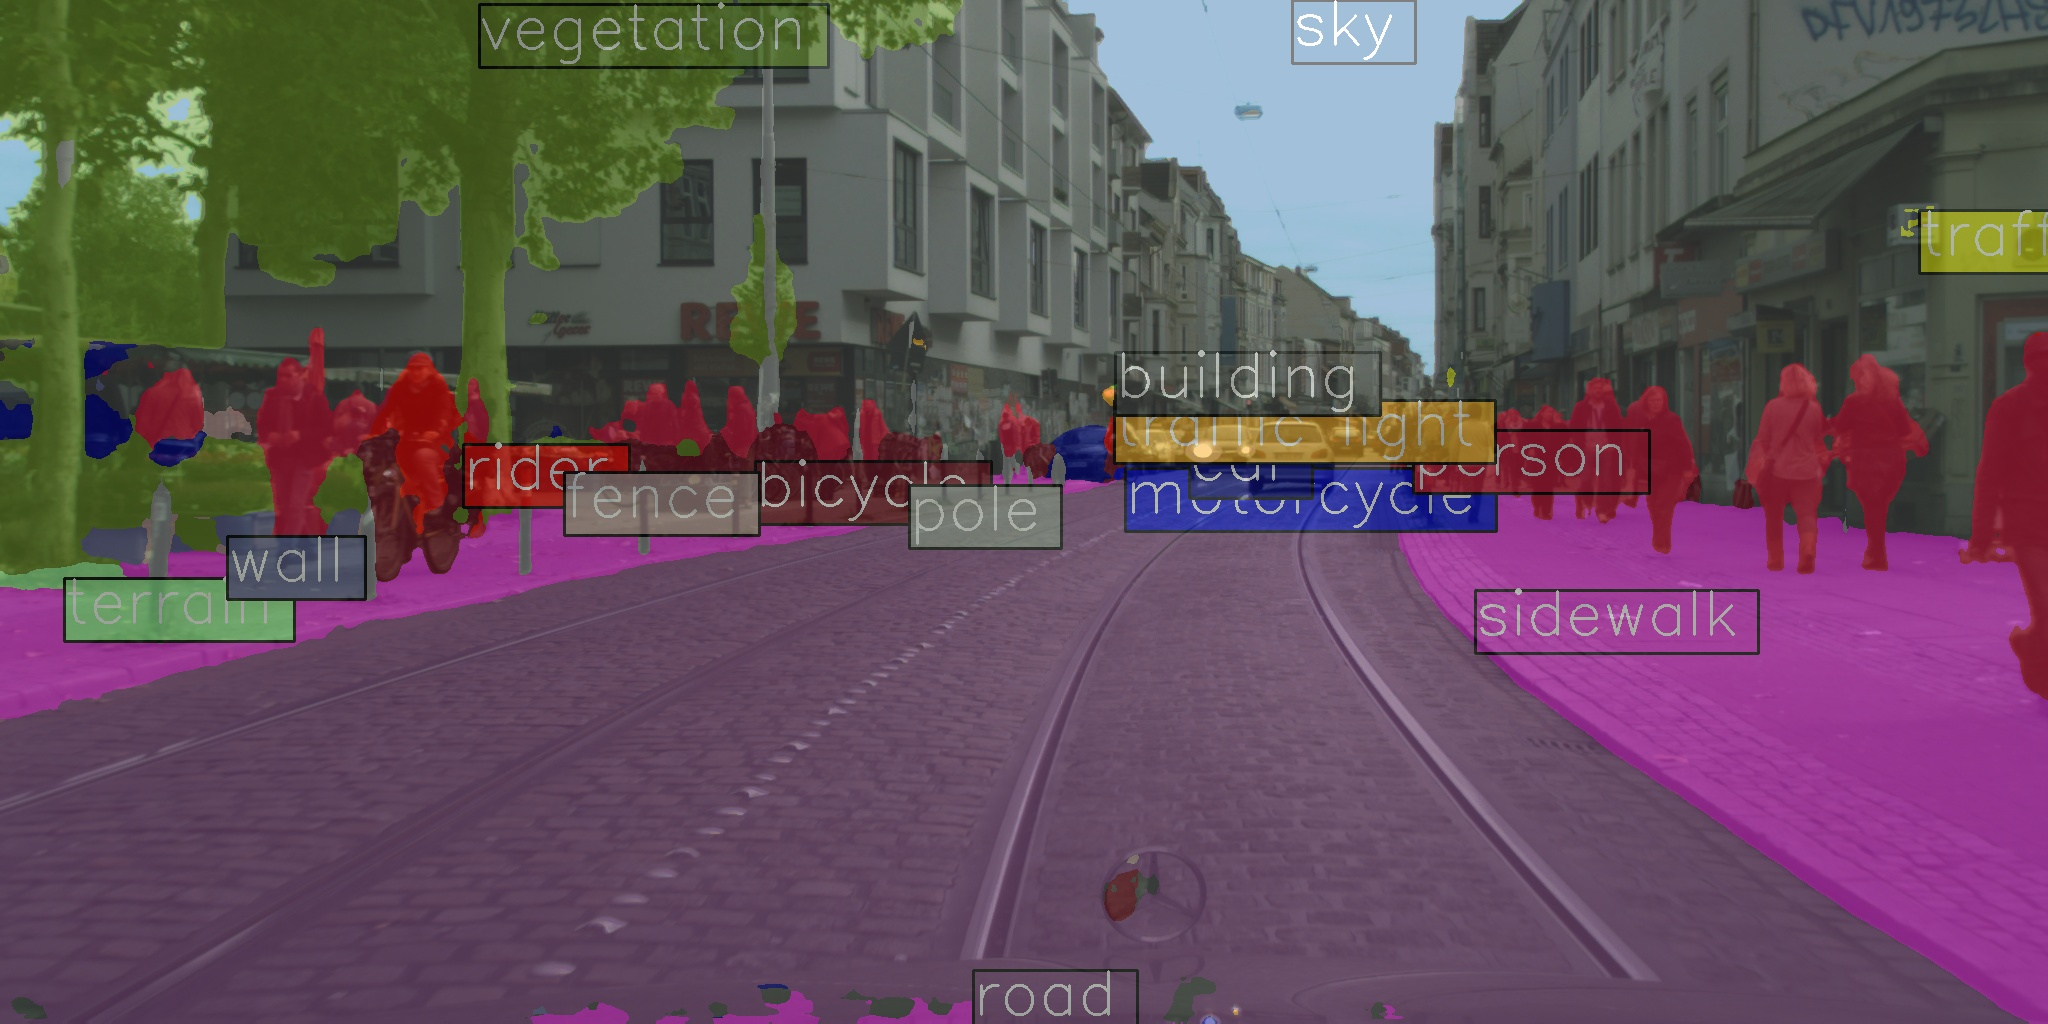
\includegraphics[width=0.49\textwidth]{result/plot/predict_1_deeplabv3plus.jpg}
    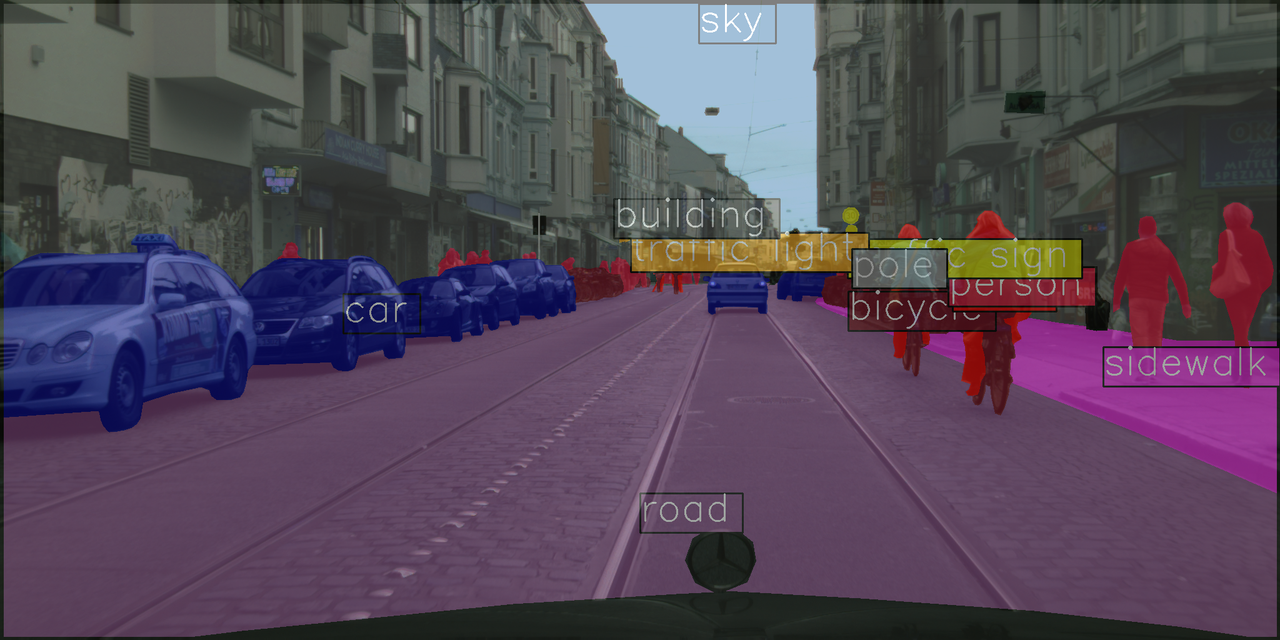
\includegraphics[width=0.49\textwidth]{result/plot/mask3.png}
    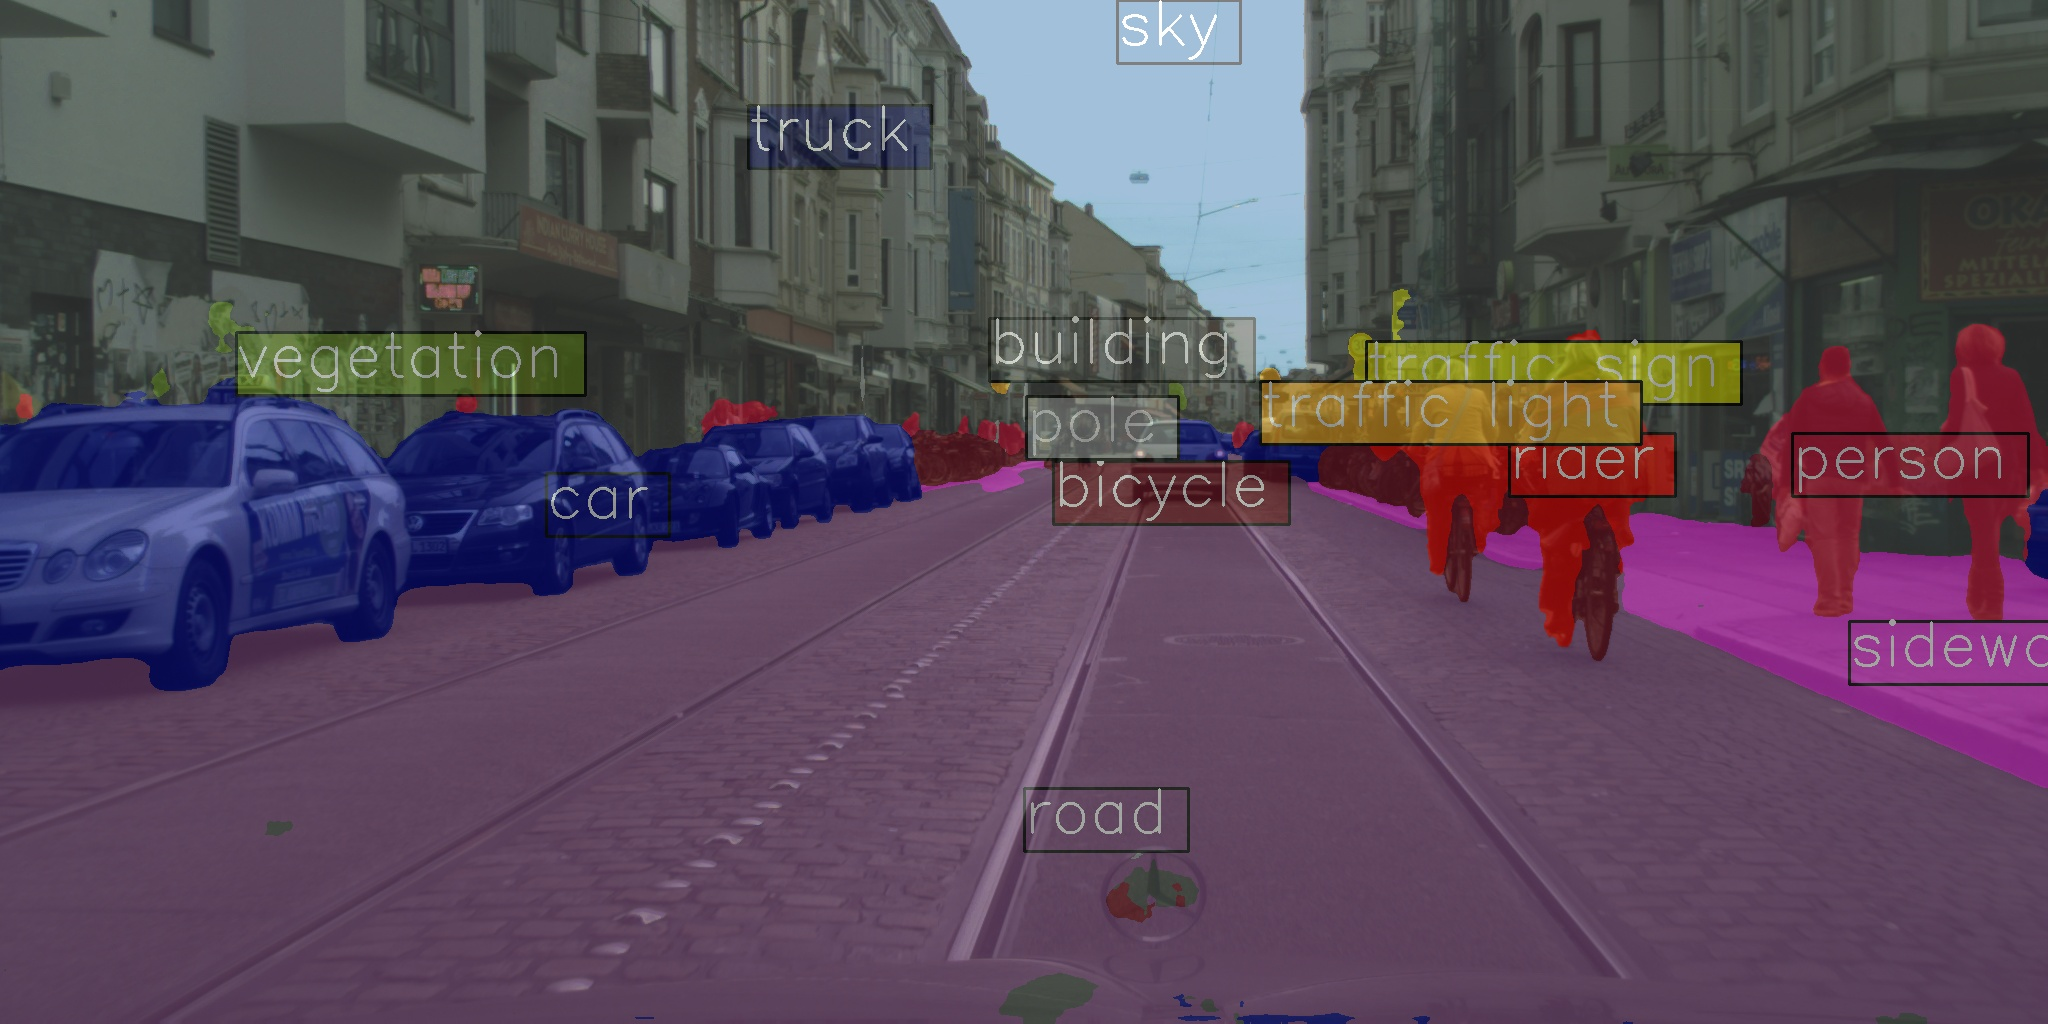
\includegraphics[width=0.49\textwidth]{result/plot/predict_2_deeplabv3plus.jpg}
    % 图片标题
    \caption{标注数据(左)和预测数据(右)对比}
    \label{fig:compare_deeplabv3plus}
\end{figure}
这个代码在mmsegmentation中没有,可以在文档中找到这段代码,并添加到文件中。这是代码所在的链接https://github.com/open-mmlab/mmsegmentation/blob/main/docs/en/user\_guides/visualization\_feature\_map.md 
wandb : https://wandb.ai/alionf-robodiff/uncategorized/runs/njilzcwj

预测的图像和原来标注的数据基本保持一致,在某些图片中分割出的物体更多,比如\ref{fig:compare_deeplabv3plus}中第二张图将单元门口上的灯检测成了路灯,\ref{fig:compare_deeplabv3plus}中第三张图将小区的窗户当成了卡车,对于自动驾驶来说,这样的检测效果并不影响车辆的行驶。如果无法完美的匹配标注的数据,那么检测出更多的物体比检测不出物体更好。
\newpage
\section{优化前后对比}
\subsubsection{尝试一:调整优化器和损失}
deeplabv3plus使用的是SGD优化器和交叉熵损失函数,我们将优化器改为AdamW,并采用组合损失的形式,在交叉熵的基础上添加FocalLoss,因为进行数据分析时得到各个类别的占比不同,采用focalloss来缓解数据分布不均衡的问题
\begin{lstlisting}[language=Python]
# 使用组合损失函数
# loss_decode=dict(type='CrossEntropyLoss', use_sigmoid=False, loss_weight=1.0)),
        loss_decode=[
            dict(type='CrossEntropyLoss', use_sigmoid=False, loss_weight=1.0),
            dict(type='FocalLoss', loss_weight=0.5, gamma=2.0, alpha=0.25)
        ],
# 更换优化器
# optimizer = dict(type='SGD', lr=0.01, momentum=0.9, weight_decay=0.0005)
optimizer = dict(type='AdamW', lr=0.001, betas=(0.9, 0.999), weight_decay=0.01)
\end{lstlisting}
结果如下:
\begin{lstlisting}[language=Python]
+---------------+-------+-------+
|     Class     |  IoU  |  Acc  |
+---------------+-------+-------+
|      road     | 97.53 |  98.9 |
|    sidewalk   | 81.78 | 89.42 |
|    building   | 90.78 | 95.04 |
|      wall     | 32.08 | 35.23 |
|     fence     |  48.6 | 64.57 |
|      pole     | 61.37 | 77.97 |
| traffic light | 65.15 | 80.14 |
|  traffic sign | 72.09 | 86.23 |
|   vegetation  | 90.76 | 96.63 |
|    terrain    | 48.42 |  53.8 |
|      sky      | 92.62 | 98.37 |
|     person    | 77.06 | 87.68 |
|     rider     |  54.4 | 74.12 |
|      car      | 91.98 | 96.04 |
|     truck     | 43.18 | 74.06 |
|      bus      | 36.22 | 40.58 |
|     train     |  7.7  |  7.9  |
|   motorcycle  | 47.69 | 61.45 |
|    bicycle    | 72.95 | 84.52 |
+---------------+-------+-------+
10/26 01:50:54 - mmengine - INFO - Iter(val) [500/500]    aAcc: 94.6500  mIoU: 63.8100  mAcc: 73.8200  data_time: 0.0112  time: 0.1686
\end{lstlisting}
mIoU还降低了3个点,效果不是很好。

\subsubsection{尝试二: 修改backbone骨干网络}
backbone将官方提供的resnet-50替换为hrnet
\begin{lstlisting}[language=Python]
model = dict(
    type='EncoderDecoder',
    data_preprocessor=data_preprocessor,
    pretrained='open-mmlab://msra/hrnetv2_w32',
    backbone=dict(
        type='HRNet',
        extra=dict(
            stage1=dict(
                num_modules=1,
                num_branches=1,
                block='BOTTLENECK',
                num_blocks=(4,),
                num_channels=(64,)),
            stage2=dict(
                num_modules=1,
                num_branches=2,
                block='BASIC',
                num_blocks=(4, 4),
                num_channels=(32, 64)),
            stage3=dict(
                num_modules=4,
                num_branches=3,
                block='BASIC',
                num_blocks=(4, 4, 4),
                num_channels=(32, 64, 128)),
            stage4=dict(
                num_modules=3,
                num_branches=4,
                block='BASIC',
                num_blocks=(4, 4, 4, 4),
                num_channels=(32, 64, 128, 256))),
        norm_cfg=norm_cfg),
    decode_head=dict(
        type='DepthwiseSeparableASPPHead',
        in_channels=256,  # HRNet最终输出通道数
        in_index=3,       # 使用HRNet的最后一个输出
        channels=512,
        dilations=(1, 12, 24, 36),
        c1_in_channels=32,  # HRNet stage2的输出通道数
        c1_channels=48,
        dropout_ratio=0.1,
        num_classes=19,
        norm_cfg=norm_cfg,
        align_corners=False,
        loss_decode=dict(type='CrossEntropyLoss', use_sigmoid=False, loss_weight=1.0),),
    auxiliary_head=dict(
        type='FCNHead',
        in_channels=128,
        in_index=2,
        channels=256,
        num_convs=1,
        concat_input=False,
        dropout_ratio=0.1,
        num_classes=19,
        norm_cfg=norm_cfg,
        align_corners=False,
        loss_decode=dict(
            type='CrossEntropyLoss', use_sigmoid=False, loss_weight=0.4)),
    train_cfg=dict(),
    test_cfg=dict(mode='whole'))  
\end{lstlisting}
结果如下:
\begin{lstlisting}
+---------------+-------+-------+
|     Class     |  IoU  |  Acc  |
+---------------+-------+-------+
|      road     | 98.04 | 98.76 |
|    sidewalk   | 84.14 | 92.99 |
|    building   | 91.68 | 96.42 |
|      wall     | 47.09 | 51.32 |
|     fence     | 59.11 | 71.92 |
|      pole     | 64.39 | 75.53 |
| traffic light | 67.52 | 77.51 |
|  traffic sign |  77.9 | 85.58 |
|   vegetation  | 92.09 | 96.87 |
|    terrain    | 60.12 | 66.58 |
|      sky      | 93.65 | 95.94 |
|     person    | 80.55 | 89.63 |
|     rider     | 59.71 | 76.24 |
|      car      | 94.11 | 97.54 |
|     truck     | 70.43 | 84.99 |
|      bus      | 64.96 | 76.05 |
|     train     | 33.13 | 35.41 |
|   motorcycle  | 46.01 | 53.64 |
|    bicycle    | 73.77 | 87.24 |
+---------------+-------+-------+
10/26 16:53:49 - mmengine - INFO - Iter(val) [500/500]    aAcc: 95.6400  mIoU: 71.5000  mAcc: 79.4800  data_time: 0.0105  time: 0.0984
\end{lstlisting}
这个结果相当不错,比原本的resnet提高了5个点,我感觉80k批次没有完全收敛,改成160k试一下。
\begin{lstlisting}
10/26 16:53:49 - mmengine - INFO - Iter(val) [500/500]    aAcc: 95.6400  mIoU: 71.5000  mAcc: 79.4800  data_time: 0.0105  time: 0.0984
\end{lstlisting}
修改为160K之后的训练效果并没有显著提升,并且在训练中期出现了mIoU的下降,之后又回升。可能是学习率设置的太高导致的。

由于160k次训练和80k的效果相近,所以后面使用80k的模型进行对比。

\subsubsection{参数量和计算量对比}
\begin{lstlisting}
==============================
Compute type: direct: randomly generate a picture
Input shape: (2048, 1024)
Flops: 1.413T
Params: 41.225M
==============================

==============================
Compute type: direct: randomly generate a picture
Input shape: (2048, 1024)
Flops: 0.431T
Params: 42.346M
==============================
\end{lstlisting}

\begin{table}[htbp]
  % \centering
  \caption{参数量和计算量对比}
  \renewcommand\arraystretch{1.4}
  \begin{tabularx}{\textwidth}{>{\centering\arraybackslash}p{1.5cm} X X}
  \toprule
  \textbf{序号} & \textbf{计算量(Flops)} & \textbf{参数量(Params)} \\
  \midrule
    1 & 1.413T & 41.225M \\
    2 & 0.431T & 42.346M \\
  \bottomrule
  \end{tabularx}
\end{table}
\subsubsection{可视化对比}
\begin{figure}[H]  % htbp表示此图片可浮动在合适位置
    \centering        % 图片居中
    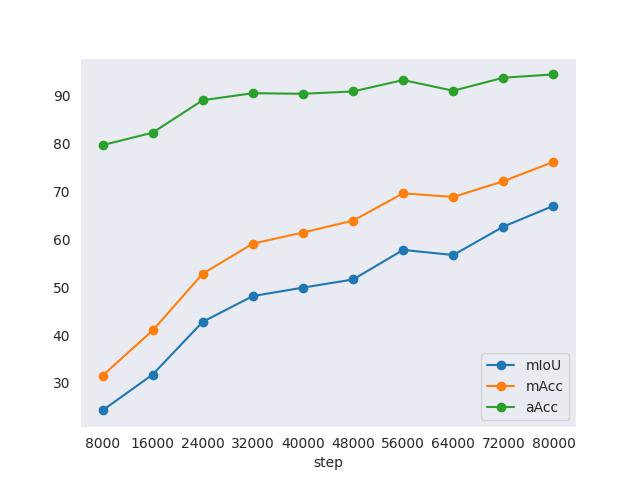
\includegraphics[width=0.49\textwidth]{result/plot/acc_deeplabv3plus.jpg}
    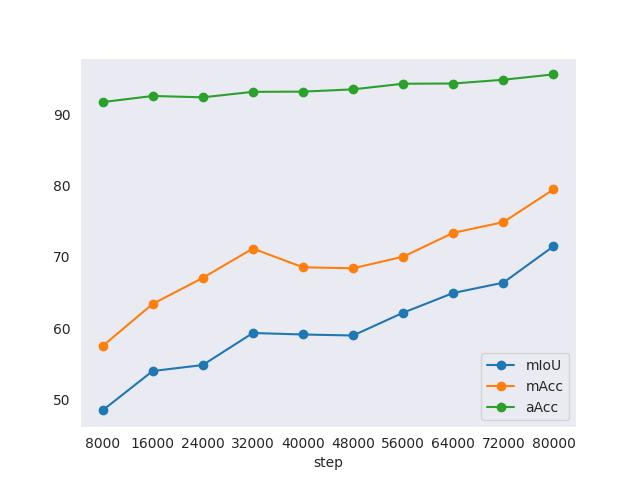
\includegraphics[width=0.49\textwidth]{result/plot/acc_deeplabv3plus_hrnet.jpg}
    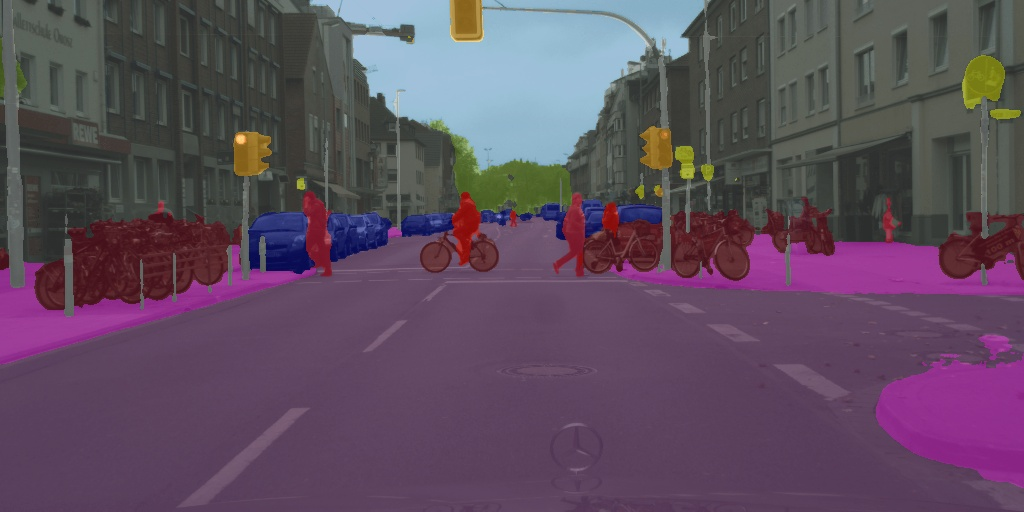
\includegraphics[width=0.49\textwidth]{result/plot/result_deeplabv3plus.jpg}
    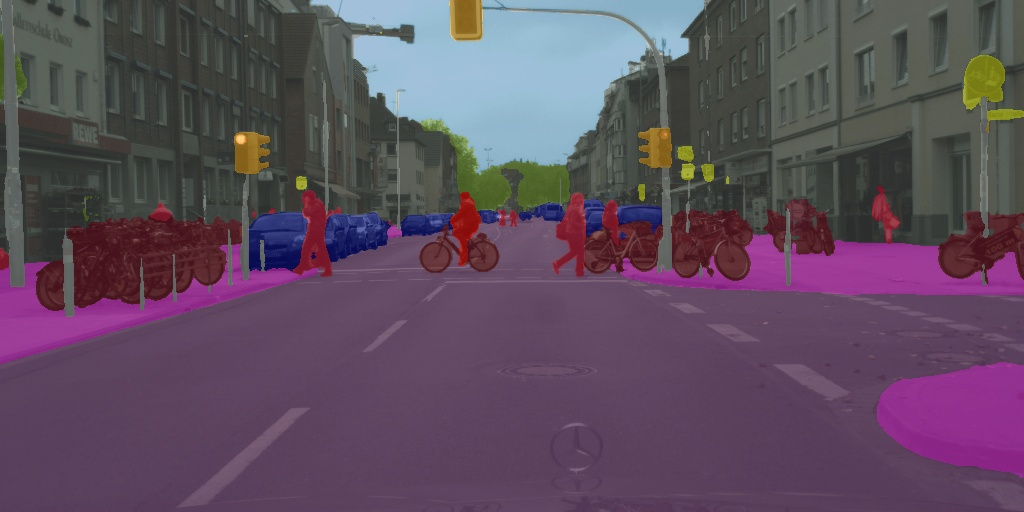
\includegraphics[width=0.49\textwidth]{result/plot/result_deeplabv3plus_hrnet.jpg}
    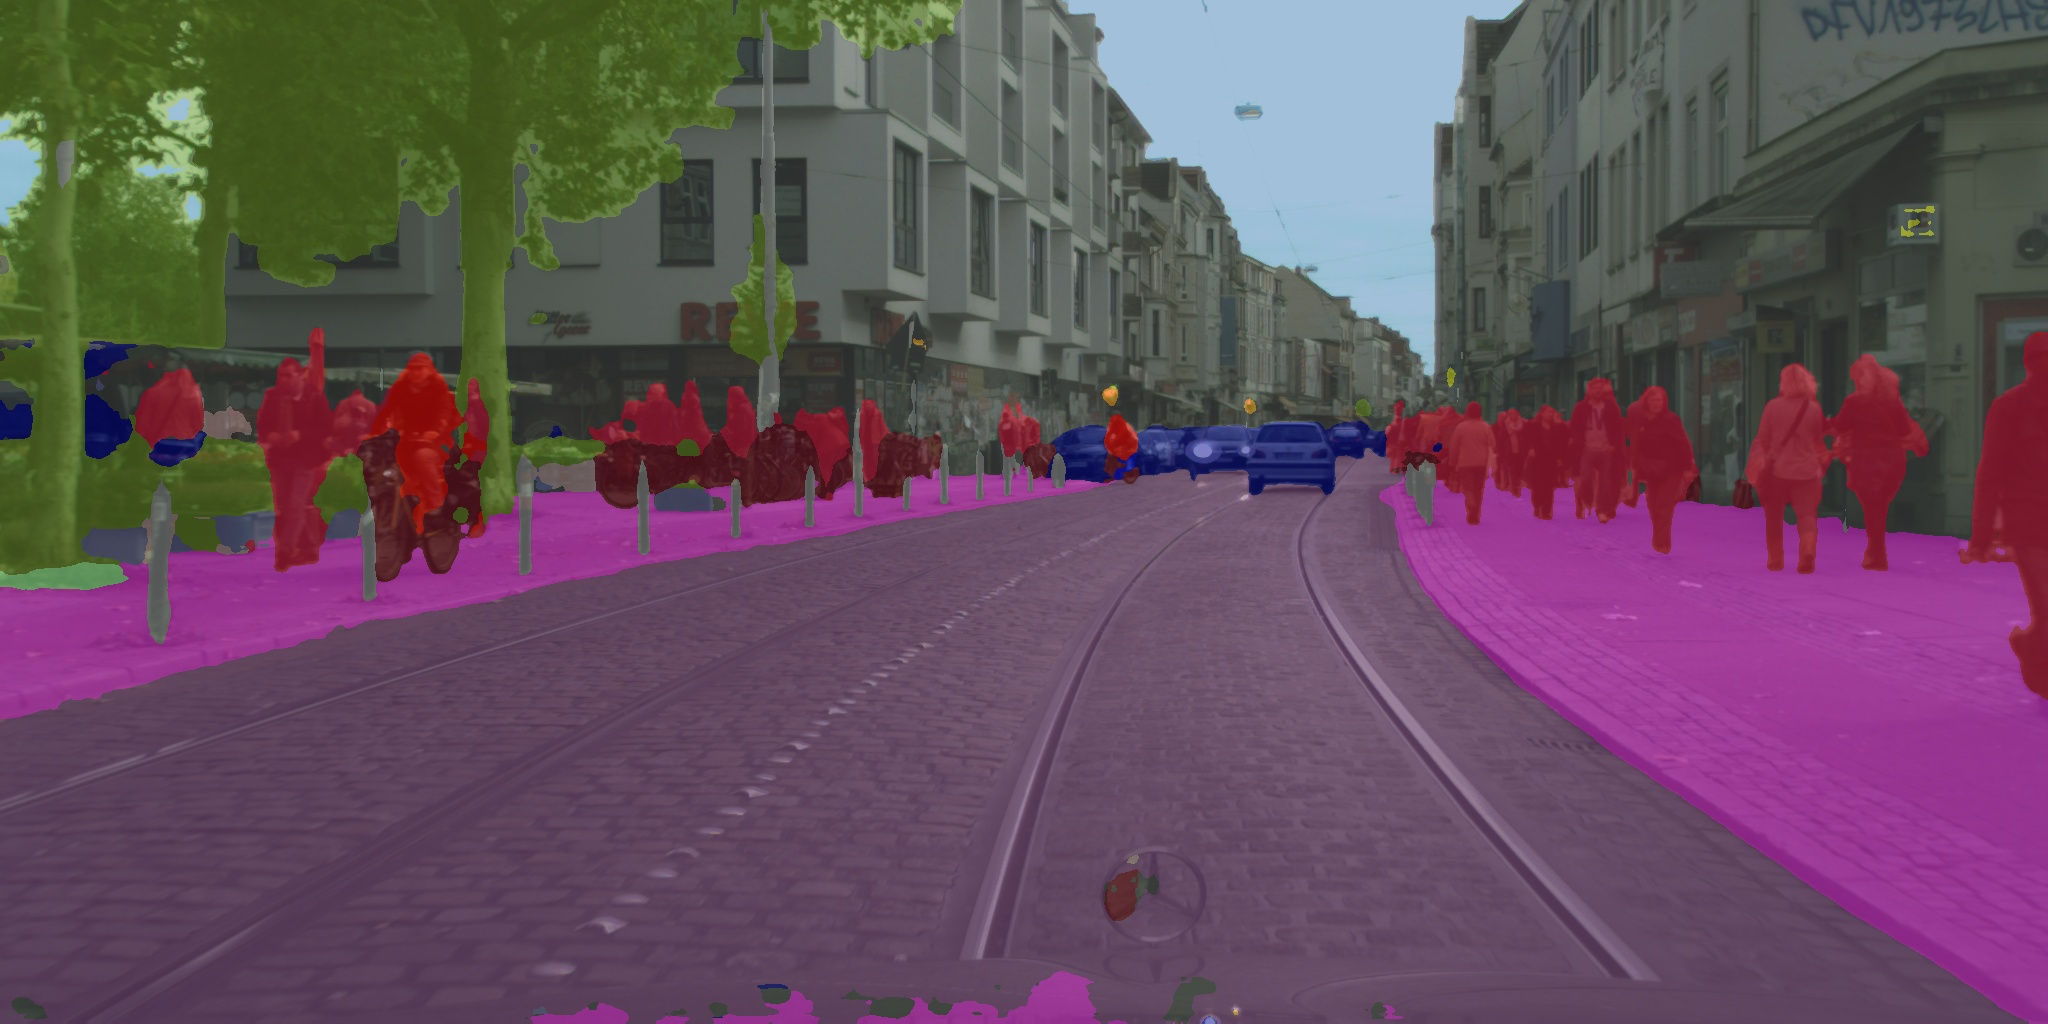
\includegraphics[width=0.49\textwidth]{result/plot/result_1_deeplabv3plus.jpg}
    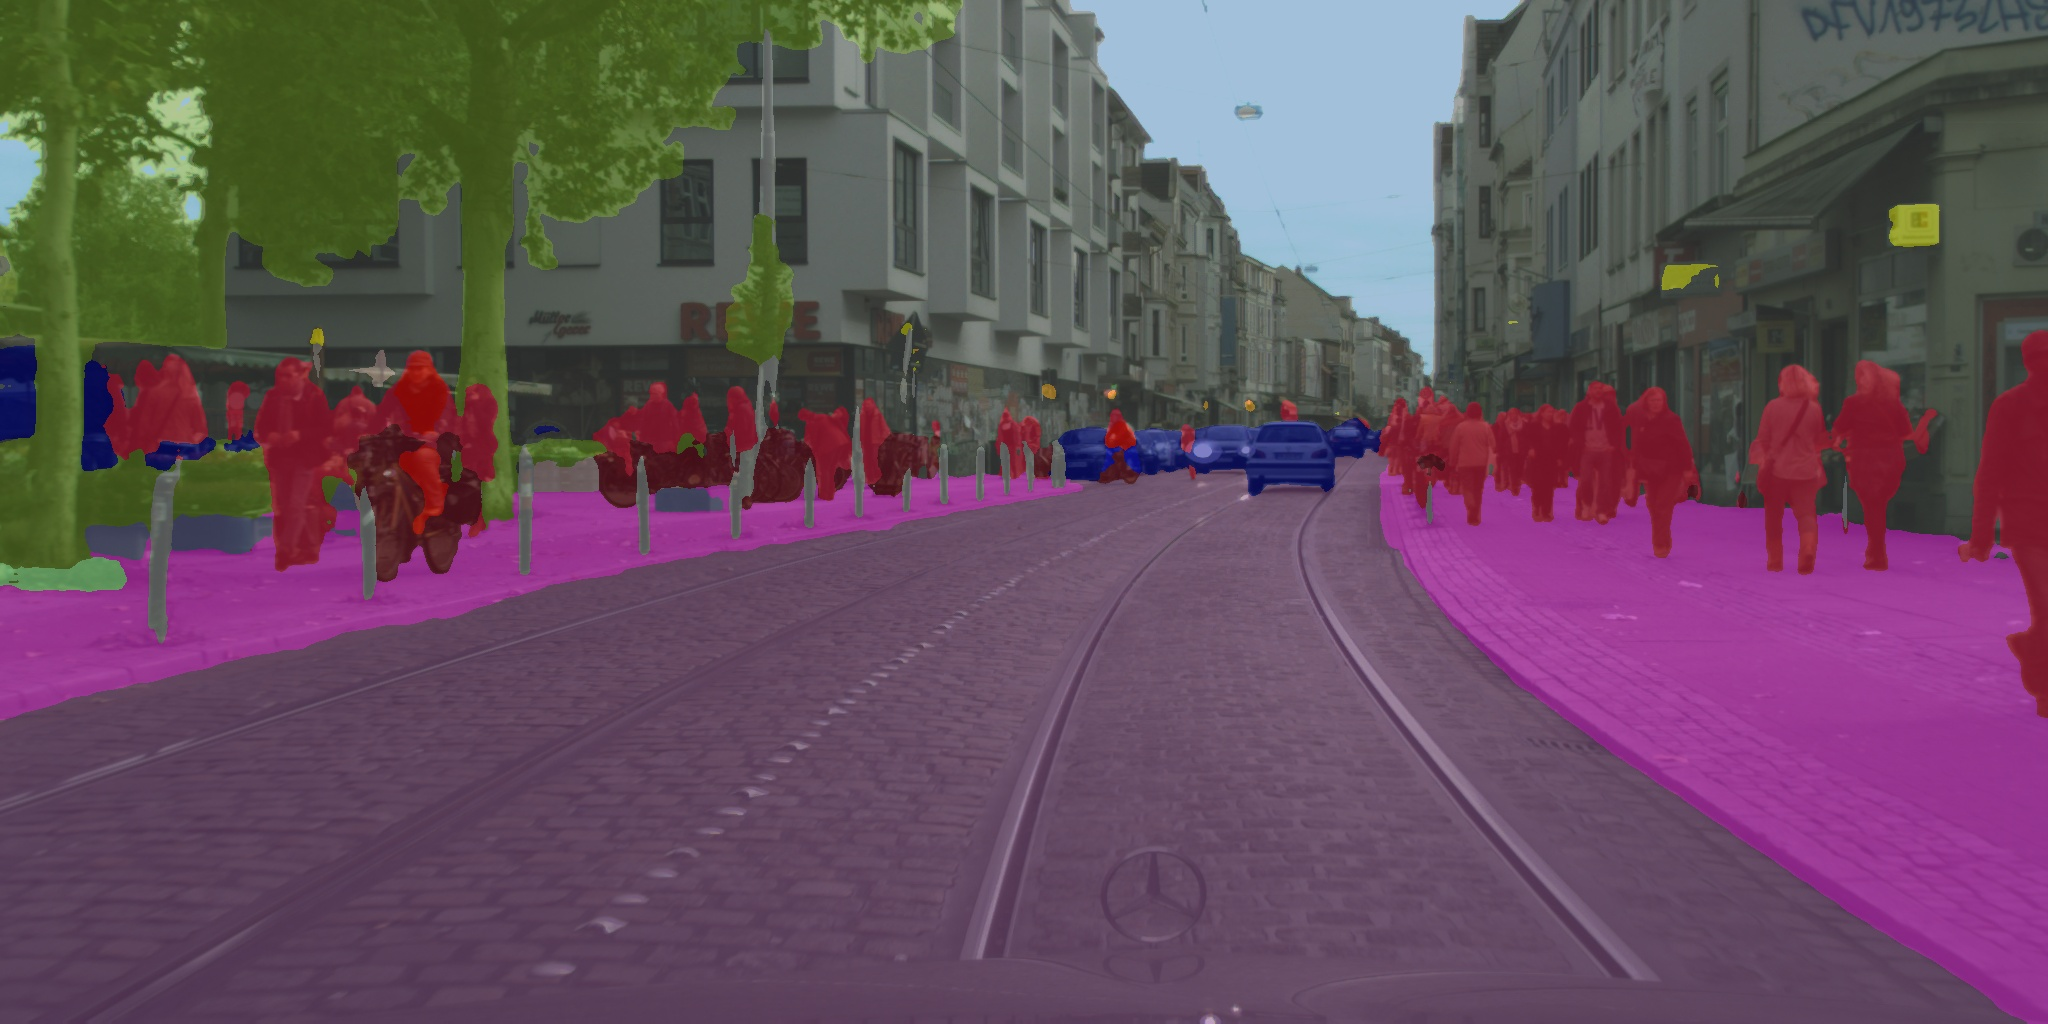
\includegraphics[width=0.49\textwidth]{result/plot/result_1_deeplabv3plus_hrnet.jpg}
    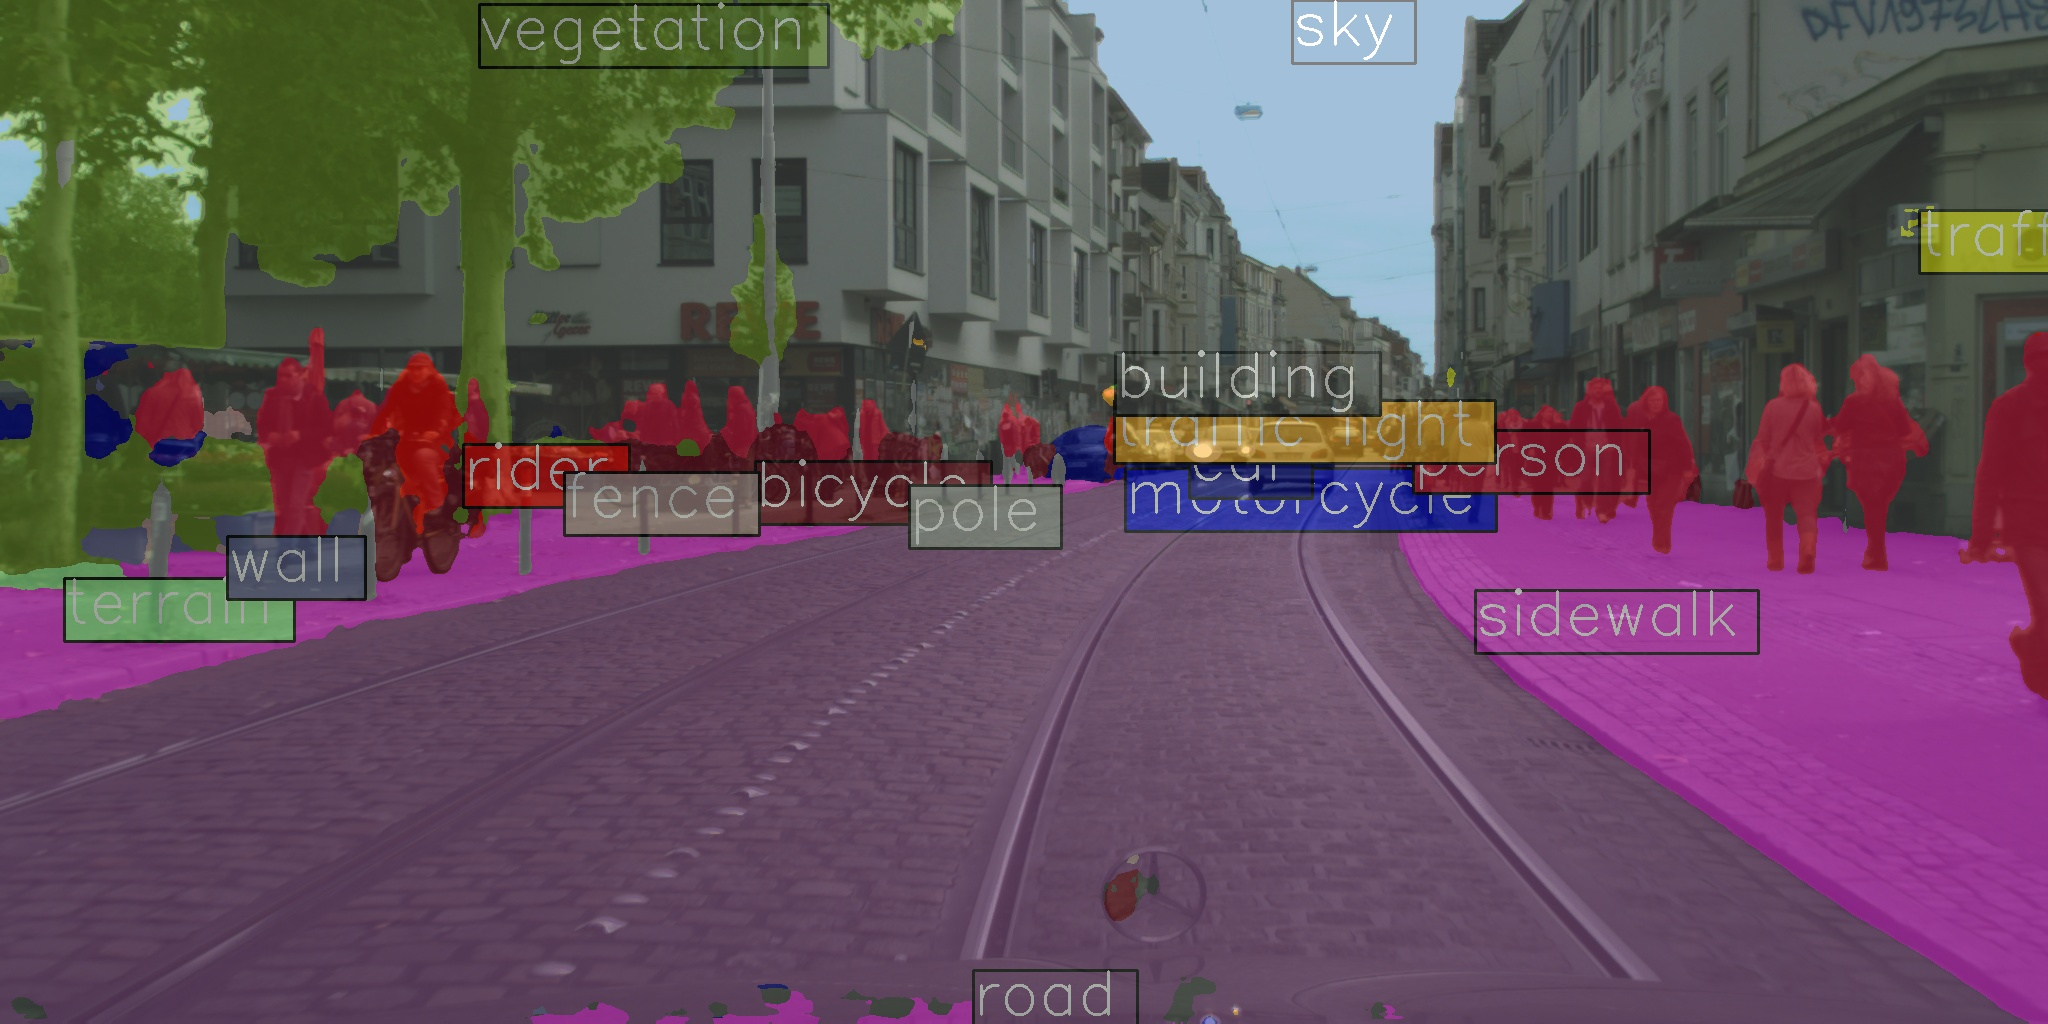
\includegraphics[width=0.49\textwidth]{result/plot/predict_1_deeplabv3plus.jpg}
    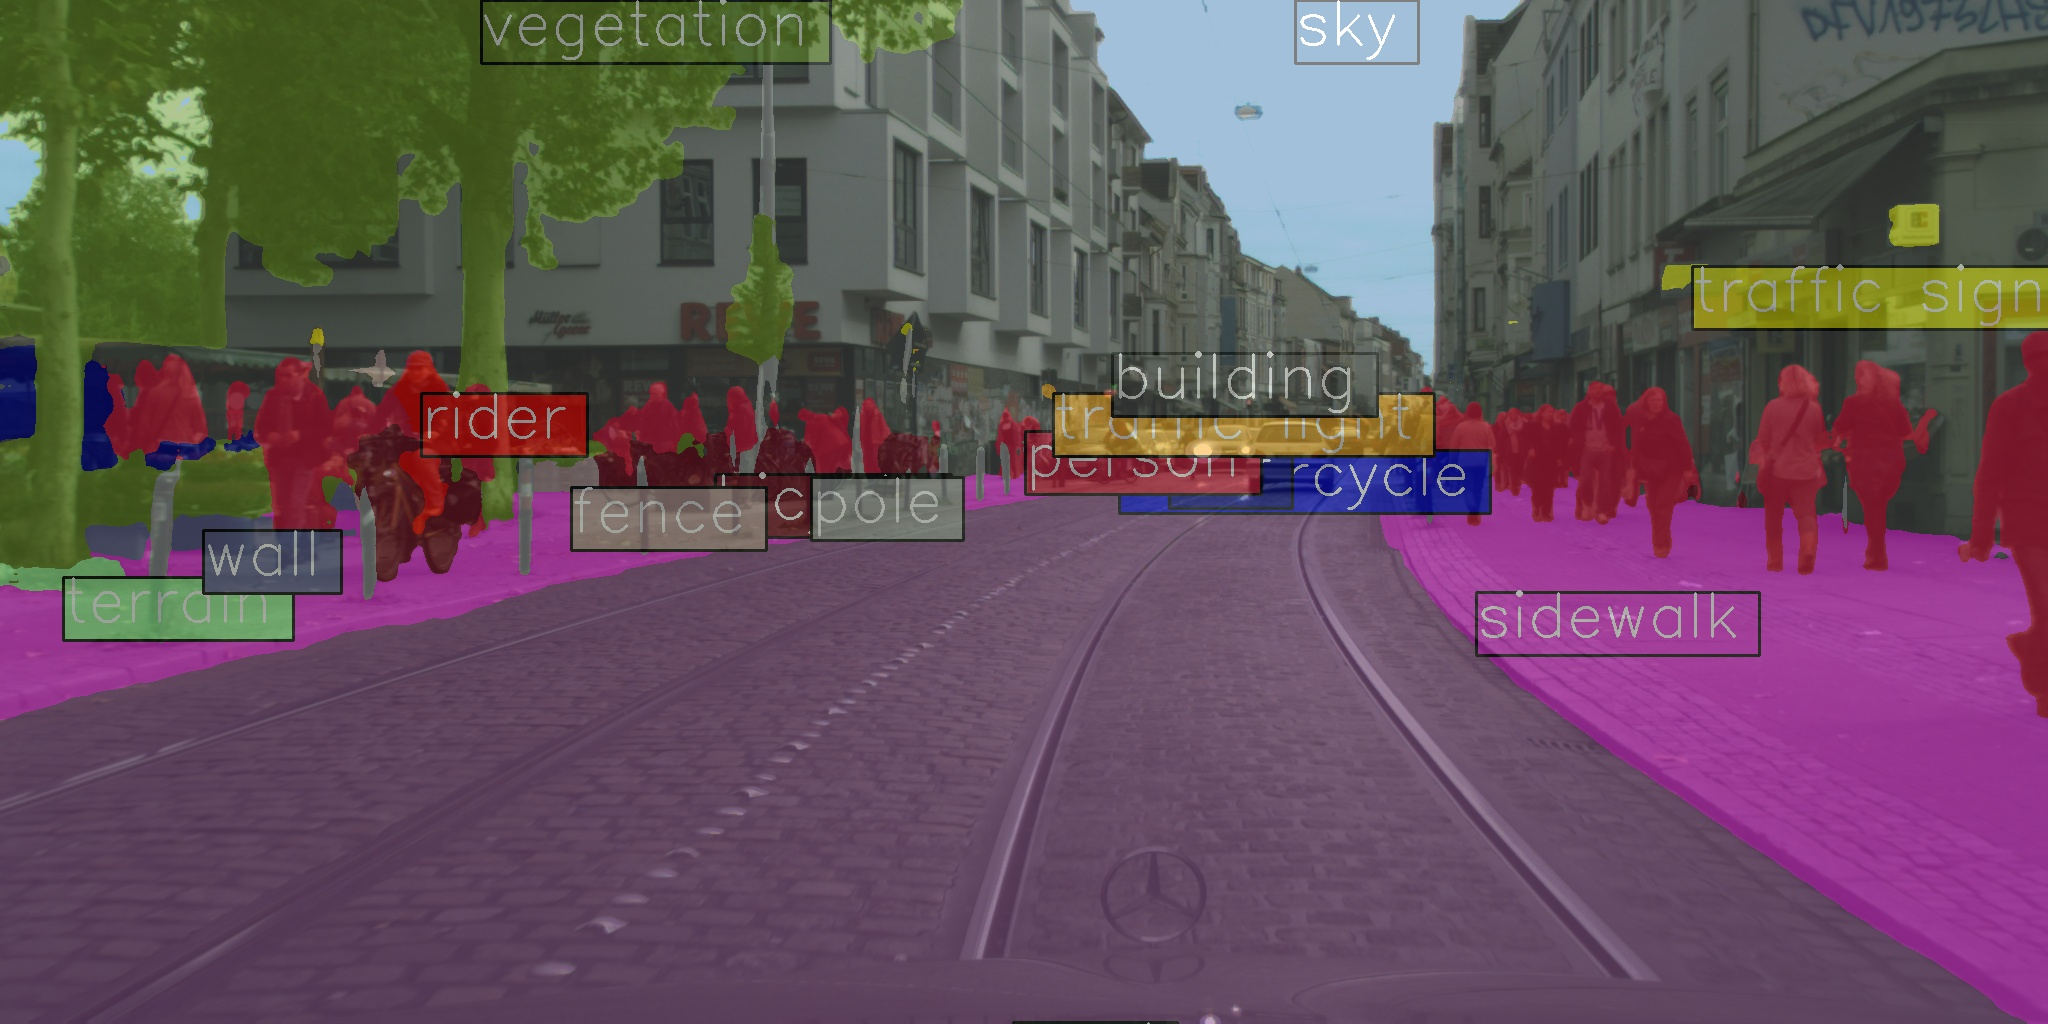
\includegraphics[width=0.49\textwidth]{result/plot/predict_deeplabv3plus_hrnet.jpg}
    % 图片标题
    \caption{resnet-r50骨干网络(左)和hrnet骨干网络(右)分割结果对比}
    \label{fig:res_hrnet_compare}
\end{figure}
从上面的结果可以看出,hrnet作为骨干网络时,mIoU提升了5个点,计算量减少了约3倍,参数量略有增加,但增加并不明显。分割结果相近。

% \begin{figure}[H]  % htbp表示此图片可浮动在合适位置
%     \centering        % 图片居中
%     \includegraphics[width=\textwidth]{result/model_struct/deeplabv3plus.onnx.png}
%     \includegraphics[width=\textwidth]{result/model_struct/deeplabv3plus_hrnet.onnx.png}
%     \caption{模型结构对比}
%     \label{fig:model_compare}
% \end{figure}

\begin{figure}[H]  % htbp表示此图片可浮动在合适位置
    \centering        % 图片居中
    \includegraphics[width=0.85\textwidth]{result/confusion_matrix/confusion_matrix.png}
    \includegraphics[width=0.85\textwidth]{result/confusion_matrix_hrnet/confusion_matrix.png}
    \caption{混淆矩阵对比resnet-r50(上)hrnet(下)}
    \label{fig:confusion_matrix_compare}
\end{figure}
观察deeplabv3plus-r50的混淆矩阵,模型对“墙”的预测效果较差,25.72\%的概率预测为建筑物(好像也没啥毛病),13.86\%概率预测为植被(观察数据集,有些植被和墙形成了相互遮挡的关系),7.83\%的概率预测为栅栏。同样的栅栏也有18.29\%的概率被预测为墙。
小汽车完全没有预测成功,按照占比排列分别预测为建筑物(36.89\%),植被(23.1\%),路(18.67\%)和杆(11.9\%),可是看预测图\ref{fig:predict_deeplabv3plus},里面有car的预测结果,不能就这一张预测到了吧!!!

\section{mask2former}
使用mask2former\_r50\_8xb2-90k\_cityscapes-512x1024.py进行训练,结果如下:
\begin{lstlisting}
+---------------+-------+-------+
|     Class     |  IoU  |  Acc  |
+---------------+-------+-------+
|      road     | 98.18 | 98.74 |
|    sidewalk   | 85.45 | 94.45 |
|    building   | 92.91 | 96.56 |
|      wall     | 53.09 | 63.58 |
|     fence     | 61.31 | 77.18 |
|      pole     | 67.98 | 78.16 |
| traffic light | 73.02 | 83.53 |
|  traffic sign | 81.03 | 87.14 |
|   vegetation  | 92.47 | 96.08 |
|    terrain    | 62.94 | 79.07 |
|      sky      | 94.81 | 98.35 |
|     person    | 83.84 | 90.99 |
|     rider     | 67.07 | 81.54 |
|      car      | 95.35 | 97.51 |
|     truck     | 76.71 | 90.54 |
|      bus      | 84.41 | 94.37 |
|     train     | 56.59 | 61.95 |
|   motorcycle  |  61.6 | 76.49 |
|    bicycle    |  79.2 | 89.25 |
+---------------+-------+-------+
2025/10/25 03:09:36 - mmengine - INFO - Iter(val) [500/500]    aAcc: 96.1600  mIoU: 77.2600  mAcc: 86.0800  data_time: 0.0103  time: 0.1363
\end{lstlisting}
mIoU比deeplabv3plus-r50高10个点,效果非常好。
\subsection{疑问}
\begin{figure}[H]  % htbp表示此图片可浮动在合适位置
    \centering        % 图片居中
    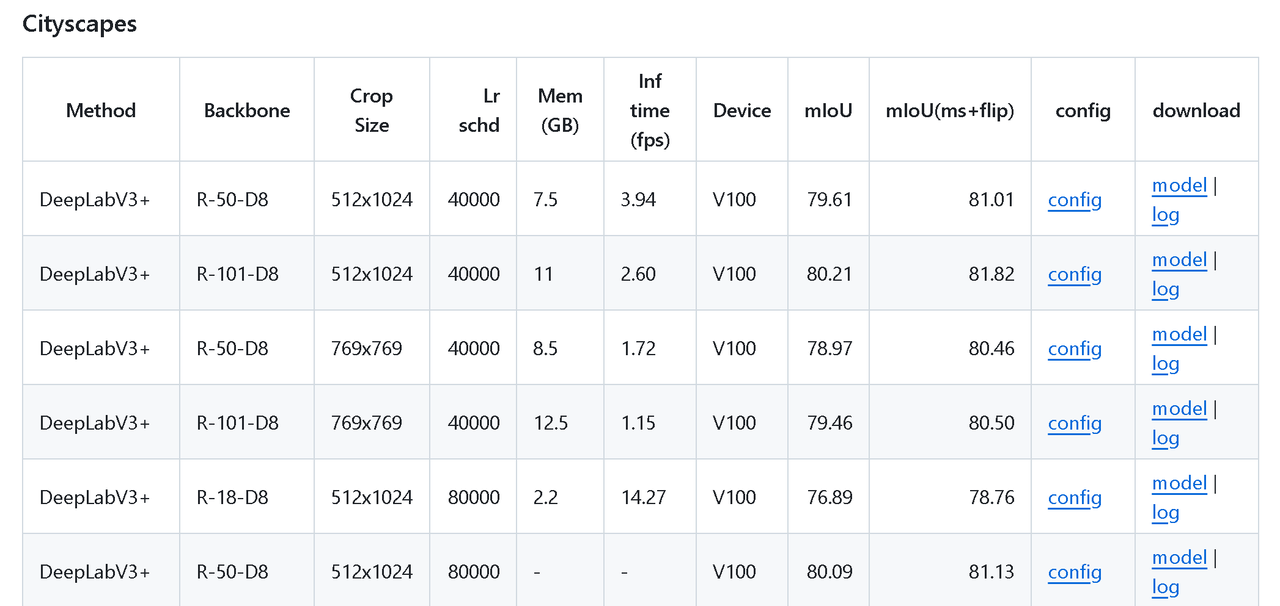
\includegraphics[width=0.95\textwidth]{result/question/deeplabv3plus.png}
    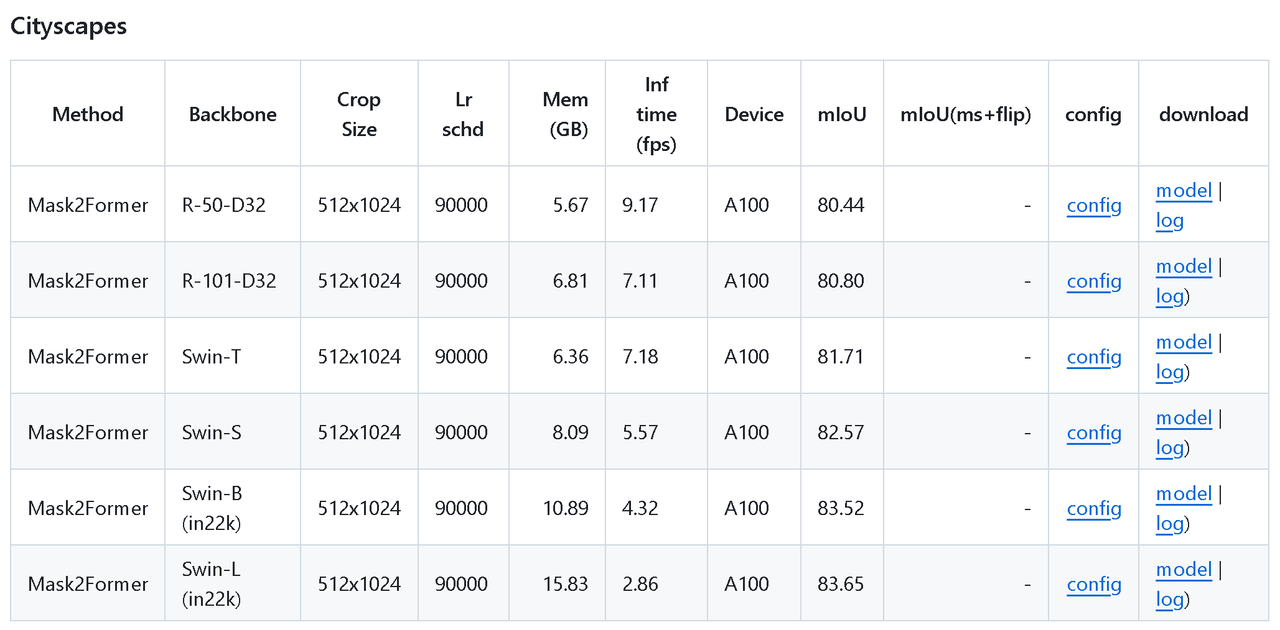
\includegraphics[width=0.95\textwidth]{result/question/mask2former.png}
    \caption{官方给出的效果deeplabv3plus(上)mask2former(下)}
    \label{fig:question}
\end{figure}

按照mmsegmentation提供的文件进行训练,得到的mIoU只有66.96,与github中给出的80.09相差很多,
而同样是官方提供的mask2former配置文件训练得到的mIoU有77.26,与标注的80.44相差并不是很多。

\section{分工}
\begin{table}[htbp]
  % \centering
  \caption{参数量和计算量对比}
  \renewcommand\arraystretch{1.4}
  \begin{tabularx}{\textwidth}{>{\centering\arraybackslash}p{1.5cm}X X}
  \toprule
  \textbf{序号} & \textbf{姓名(Name)} & \textbf{分工(Works)} \\
  \midrule
    1 & 胡 &  deeplabv3plus训练与优化 \newline 文档 \newline 模型结构可视化 \newline 绘制混淆矩阵\\
    2 & 姜 &  数据分析\newline mask2former训练 \newline 模型结果可视化 \newline PPT制作 \\
  \bottomrule
  \end{tabularx}
\end{table}
\section{总结与展望}

\end{document}

